\documentclass[11pt]{article}
\usepackage{amsmath, amssymb, graphicx}
\usepackage{booktabs}
\usepackage{subcaption}
\usepackage{siunitx}
\sisetup{detect-all}
\usepackage[round]{natbib}
\title{A Benchmark Dataset for Satellite-Based Estimation and Detection of Rain}
\author{%
	Simon Pfreundschuh\textsuperscript{1}, %
	Malarvizhi Arulraj\textsuperscript{2}, %
	Ali Behrangi\textsuperscript{3}, %
	Linda Bogerd\textsuperscript{3}, \\
	Alan James Peixoto Calheiros\textsuperscript{3}, %
	Daniele Casella\textsuperscript{3}, %
	Neda Dolatabadi\textsuperscript{3}, \\ %
	Clement Guilloteau\textsuperscript{2}, %
	Jie Gong\textsuperscript{3}, %
	Pierre Kirstetter\textsuperscript{3}, %
	GyuWon Lee\textsuperscript{3}, \\ %
	Maximilian Maahn\textsuperscript{3}, %
	Lisa Milani\textsuperscript{3}, %
	Rayana Palharini\textsuperscript{3},\\%
	Veljko Petković\textsuperscript{3}, %
	Soorok Ryu\textsuperscript{3}, %
	Paolo Sanò\textsuperscript{3}, %
	Jackson Tan\textsuperscript{3}\\
}
\date{
  \begin{flushleft}
	\footnotesize
	\textsuperscript{1} Department of Atmospheric Science, Colorado State University \\
	\textsuperscript{2} Department of Civil and Environmental Engineering, University of California Irvine \\
	\textsuperscript{3} Department of Hydrology and Atmospheric Sciences, University of Arizona\\
	\textsuperscript{2} Department of Mathematics, University B, City, Country \\
	\textsuperscript{3} Department of Atmospheric Science, Colorado State University \\
	\textsuperscript{4} Instituto Nacional de Pesquisas Espaciais \\
	\textsuperscript{5} Department of Atmospheric Sciences, Kyungpook National University \\
	\textsuperscript{5} Department of Atmospheric Sciences, Kyungpook National University \\
	\textsuperscript{6} NASA Goddard Space Flight Center \\
	\textsuperscript{7} University of Maryland, Baltimore County \\
	\textsuperscript{7} University of Maryland\\
	\textsuperscript{8} Institute for Meteorology, University of Leipzig \\
	\textsuperscript{9} Institute of Atmospheric Sciences and Climate, Italian National Research Council \\
	\textsuperscript{10} Earth System Science Interdisciplinary Center, University of Maryland  \\
	\textsuperscript{10} Cooperative Institute for Satellite Earth System Studies, University of Maryland  \\
	\end{flushleft}
}

\begin{document}
\maketitle


\begin{abstract}

Accurately monitoring the global distribution and evolution of precipitation is
essential for understanding precipitation processes and improving forecasts.
Satellite observations remain the only means of achieving consistent,
global-scale precipitation monitoring. While machine learning has long been
applied to satellite-based precipitation retrieval, the absence of a
standardized benchmark dataset has hindered fair comparisons between methods and
limited progress in algorithm development.

To address this gap, the International Precipitation Working Group has developed
SatRain, the first AI-ready benchmark dataset for satellite-based detection and
estimation of rain, snow, graupel, and hail. SatRain includes multi-sensor
satellite observations representative of the major platforms currently used in
precipitation remote sensing, paired with high-quality reference estimates from
ground-based radars corrected using rain gauge measurements. It offers a
standardized evaluation protocol to enable robust and reproducible comparisons
across machine learning approaches.

In addition to supporting algorithm evaluation, the diversity of
sensors and inclusion of time-resolved geostationary observations make SatRain a
valuable foundation for developing next-generation AI models to deliver more
accurate, detailed, and globally consistent precipitation estimates.

\end{abstract}

\section{Background and Summary}

Precipitation, the deposition of water in liquid or frozen form from the
atmosphere onto the Earth's surface, is essential for sustaining ecosystems and
a wide range of human activity. However, extreme events at both ends of the
climatological distribution of precipitation, such as droughts or heavy
precipitation, can cause substantial damage to societies and human livelihoods.
Monitoring the global distribution of precipitation is therefore critical not
only for advancing scientific understanding of the processes that shape
precipitation patterns and drive extreme events but also economic planning and
civil security. Despite its crucial role in many aspects of economic and social
life on Earth, precipitation estimation still faces significant challenges in
meeting the needs of hydrological and climate research, as well as operational
applications. Precipitation is one of the most difficult atmospheric parameters
to measure accurately because its estimation from both satellite and ground-based
observations is complicated by several factors: its high spatial and temporal
variability; its phase (liquid, solid, or mixed); its microphysical compositions
(,e.g., particle shape, densities, and sizes); and the difficulties involved
in converting radiometric measurements into quantitative precipitation
estimates \citep{Levizzani2020Satellite}.

Satellite-based remote sensing is an essential tool for monitoring precipitation
continuously on a global scale. Rain gauges provide valuable direct
measurements, but their coverage is largely confined to continental land masses
and is often irregularly distributed \citep{Kidd2017RainGauges}. In addition,
because gauges measure precipitation only at a single point, they cannot
adequately represent the spatial structure of rainfall systems. Ground-based
weather radars yield spatially-continuous estimates at high spatial resolution
but their coverage remains geographically limited. In contrast, satellites offer
consistent, near-global observations, making them the only means of obtaining
continuous and spatially comprehensive estimates of precipitation.

However, the accuracy with which precipitation can be estimated or detected from
satellite observations varies significantly with sensor type and observing
conditions \citep{Stephens2007RemoteSensing}. Although a small number of
precipitation radars have been deployed to measure precipitation from space,
their spatial and temporal coverages are severly limited. Therefore, global
precipitation monitoring has to rely mostly on passive sensors. Passive
microwave sensors operating in the 10-89 GHz range can detect emission signals
associated with precipitation particles over the ocean. However, over land the
emission signal from precipitation is hardly distinguishable from the high and
variable emission signal from the surface. While higher microwave frequencies (>
89 GHz) are less sensitive to surface properties, their information content
primarily derives from scattering by large rain drops and ice particles
\citep{Bennartz2003Sensitivity}, providing a weaker link to the precipitation at
the surface. Furthermore, the spatial resolution achievable with passive
microwave sensors is limited, requiring deployment in low-Earth orbits. As a
result, even for satellite missions comprising constellations of multiple
sensors, such as the Global Precipitation Measurement (GPM) mission
\cite{Hou2014GPMMission}, the revisit times can exceed three hours in the
tropics (30 °S - 30 °N).

By contrast, geostationary satellites offer near-continuous temporal coverage
over much of the globe, with spatial resolutions on the order of a few
kilometers. Their main limitation is that they operate only in the visible and
infrared bands, which are primarily sensitive to the cloud tops and therefore
provide an even less direct link to surface precipitation than passive microwave
observations.

\begin{figure}[htbp]
	\centering
	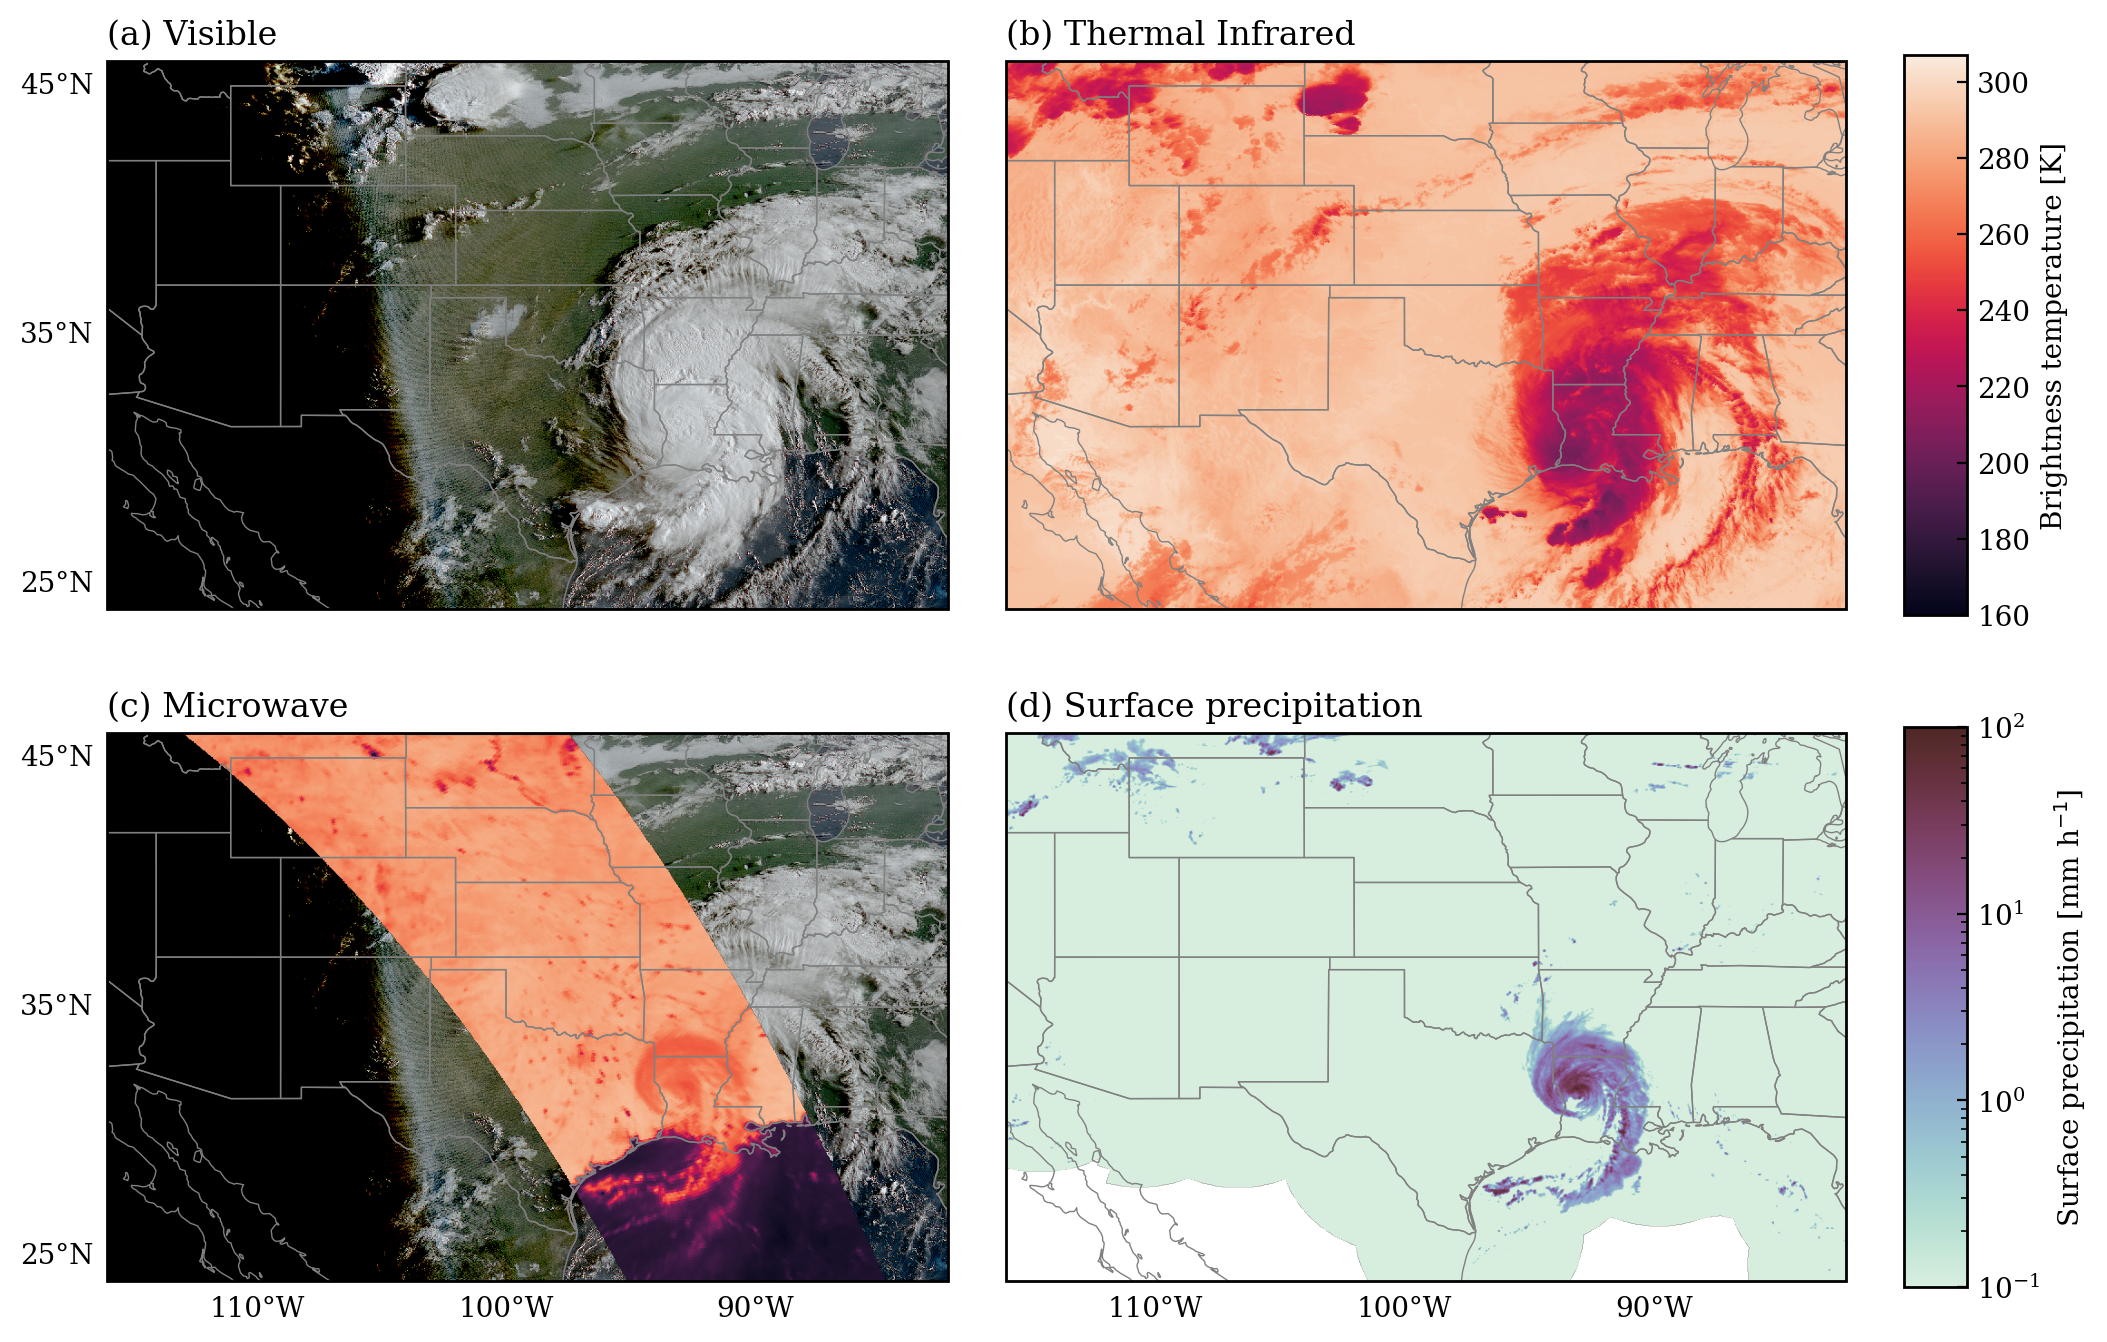
\includegraphics[width=1.0\textwidth]{figures/fig01}
	\caption{Satellite observations and surface precipitation estimates for Hurricane Laura on August 27, 2020, at 12:41 UTC. Panel (a) shows a true-color composite from the Advanced Baseline Imager (ABI) aboard the GOES-16 geostationary satellite. Panel (b) displays globally available thermal infrared imagery at $\SI{11}{\micro \meter}$  derived from a constellation of geostationary satellites. Panel (c) presents passive microwave observations from the GPM Microwave Imager (GMI) 36.5-GHz, horizontally-polarized channel, overlaid on the GOES true-color RGB. Panel (d) depicts surface precipitation rate estimates from NOAA’s Multi-Radar Multi-Sensor product.}
	\label{fig:observations_conus}
\end{figure}

Figure~\ref{fig:observations_conus} illustrates the key characteristics of the
various types of satellite observations used for the remote sensing of
precipitation. Panel (a) presents a true-color composite from the Advanced
Baseline Imager (ABI, \citeauthor{Schmit2005Introducing},
\citeyear{Schmit2005Introductin}) aboard GOES-16, showing Hurricane Laura as an
expansive cloud system in the southeastern portion of the domain. Visible
imagery such as this true-color composite can reveal detailed cloud structures
but is limited to daylight hours due to its reliance on reflected sunlight.
Panel (b) displays thermal infrared (IR) imagery with a wavelength of
\SI{11}{\micro \meter} observed from a geostationary platform. At this
wavelength, the clear-sky atmosphere exhibits high transmittance, while clouds
are opaque. Consequently, the measured radiances primarily originate from the
Earth’s surface in cloud-free regions and from cloud tops in cloudy regions. Due
to the vertical thermal structure of the atmosphere, the cloud tops appear as
areas of cold brightness temperatures against a relatively warmer background.
Panel (c) shows horizontally-polarized passive microwave observations at a
frequency of $\SI{36.5}{\giga \hertz}$, corresponding to a wavelength of around
$\SI{8}{\milli \meter}$. Surface-sensitive passive microwave observations are
characterized by a strong contrast between ocean and land surfaces. Over the
radiatively cold ocean background, Hurricane Laura's rainband appears as a
region of enhanced brightness temperature due to emission from liquid
hydrometeors. Over land, the surface itself emits strongly at microwave
frequencies, making it difficult to isolate the emission signal from raindrops.
Instead, precipitation is primarily detected through the scattering signature of
large raindrops and ice particles, which reduce the observed brightness
temperatures by attenuating surface emission.

Comparing the three panels to the corresponding radar-based surface
precipitation estimates underscores the strength of passive microwave
observations: while visible and IR imagery primarily depict cloud-top features
that may not correlate with surface rainfall, microwave observations exhibit
higher spatial coherence with surface precipitation. The principal limitation of
passive microwave imagery, however, is its limited spatiotemporal coverage due
to narrower swath widths, longer revisit times, and lower spatial resolution.

\subsection{From Satellite Observations to Precipitation Estimates}


Satellite observations only contain an indirect signal from the near-surface
precipitation and thus require careful processing to produce reliable surface
precipitation estimates. This conversion of satellite measurements into
precipitation estimates is commonly referred to as retrieval. While a
physics-based formulation of precipitation retrieval algorithms is possible,
practical implementations typically require a range of simplifications and
ad-hoc assumptions, such as normally distributed retrieval targets and
measurement errors or close-to linear relationships between atmospheric
variables and satellite observations \citep{Boukabara2011MiRS,
  Kummerow2015GPROF, Maahn2020OptimalEstimation}. Because of these difficulties,
purely empirical approaches have long been used to directly relate satellite
observations to precipitation estimates obtained from other measurement
techniques \citep{ Griffith1978, Adler1988InfraredRainfall,
  Hong2004Precipitation}. The rise of machine learning (ML) and more recent AI
techniques have led to the development of a range of new ML-based
algorithms that yield promising results \citep{Sadeghi2019Persiann,
  Pfreundschuh2022BrazilRetrieval, Pfreundschuh2022Gprof, Gorooh2023LEOGEO}.


\subsection{The Need for a Unified Benchmark Dataset}

The number of ML-based satellite precipitation retrievals is
growing \citep{Sano2018PNPR, Amell2025Probabilistic}, however the algorithms
described in the literature are difficult to compare. This is largely because
they are typically developed for specific sensors, regions, time periods, and
even resolutions. Given the high spatiotemporal variability of precipitation,
such differences in sampling and geographic focus significantly influence
accuracy metrics, rendering published results incomparable. Moreover, the
performance of empirical retrieval algorithms is influenced by the volume,
quality, and spatiotemporal sampling of the training and evaluation data, and
thus does not solely reflect the intrinsic qualities of a specific algorithm or
model.

This lack of comparability makes it difficult to isolate algorithmic
improvements driven by advancements in ML from differences
introduced by the choice of training and evaluation data. To address this
challenge, the International Precipitation Working Group (IPWG), a permanent
Working Group of the Coordination Group for Meteorological Satellites (CGMS),
has established a ML working group tasked with developing a
standardized benchmarking dataset for empirical and ML-based
precipitation retrievals \citep{Kubota2025IPWG}. The result of this effort is
the Satellite-Based Estimation and Detection of Rain (SatRain) dataset, an
AI-ready, large-scale benchmark dataset for the development and evaluation of
precipitation retrieval algorithms covering a wide range of observations
modalities and multiple climate zones. Despite its name, the dataset is not
limited to rain but includes all types of precipitation encountered during the
training and testing periods thus providing a comprehensive resource for
developing and testing precipitation retrieval algorithms.


\subsection{The SatRain Dataset}

The SatRain dataset integrates multi-sensor satellite observations with
gauge-corrected, ground-based radar precipitation estimates. It provides a
large, curated training set over the continental United States (CONUS),
encompassing diverse climate regimes ranging from subtropical humid regions to
arid deserts, mountainous terrain, and temperate to cold continental zones. Data
are available both on a 0.036-degree regular latitude–longitude grid and the native
sampling of the passive microwave sensors. All input and reference fields are
consistently mapped to these two spatial representations, enabling direct use
for both pixel-based and image-based AI algorithms and ensuring the dataset’s
AI-readiness. The satellite observations span a wide range of sensing modalities
relevant to precipitation remote sensing, including temporally resolved imagery
from geostationary platforms. To support model generalization studies, SatRain
also includes independent test sets from Korea and Austria, covering distinct
climate regimes and incorporating alternative reference measurement techniques.

\section{Methods}

\subsection{Data Sources}

The SatRain dataset integrates four principal data sources:

\begin{enumerate}
  \item PMW sensors,
  \item geostationary sensors,
  \item ancillary environmental data,
  \item reference precipitation estimates from ground-based weather radar networks over CONUS,
  \item independent precipitation estimates from ground-based radars over Korea and gauge measurements in Austria.
\end{enumerate}

Since PMW observations over a given region of interest are limited to discrete
overpass times, the dataset is constructed around the overpasses of PMW sensors
to which data from the other sources is added accordingly.

A key challenge in creating the SatRain dataset was reconciling differences in
spatial resolution and sampling across sensors. To balance flexibility with
manageable dataset size, SatRain data is provided in two sampling geometries.
The gridded data is mapped to a shared, regular latitude-longitude grid at
\SI{0.036}{\degree} resolution. This resolution matches the native grid of a
major global geostationary IR dataset \citep{NCEP_CPC_L3_IR} and remains finer
than the effective resolution of current satellite precipitation estimates. In
addition to that, the on-swath dataset is kept on the native spatial sampling of
the PMW base sensor. Because many precipitation retrieval algorithms have
historically been developed on the native sensor sampling, SatRain retains this
format to support these retrieval designs and cross-comparison against existing
operational retrievals such as the Goddard Profiling Algorithm
\citep{Kummerow2015GPROF}.

\subsubsection{PMW Sensors}

\begin{figure}[htbp] % h=here, t=top, b=bottom, p=page of floats
	\centering
	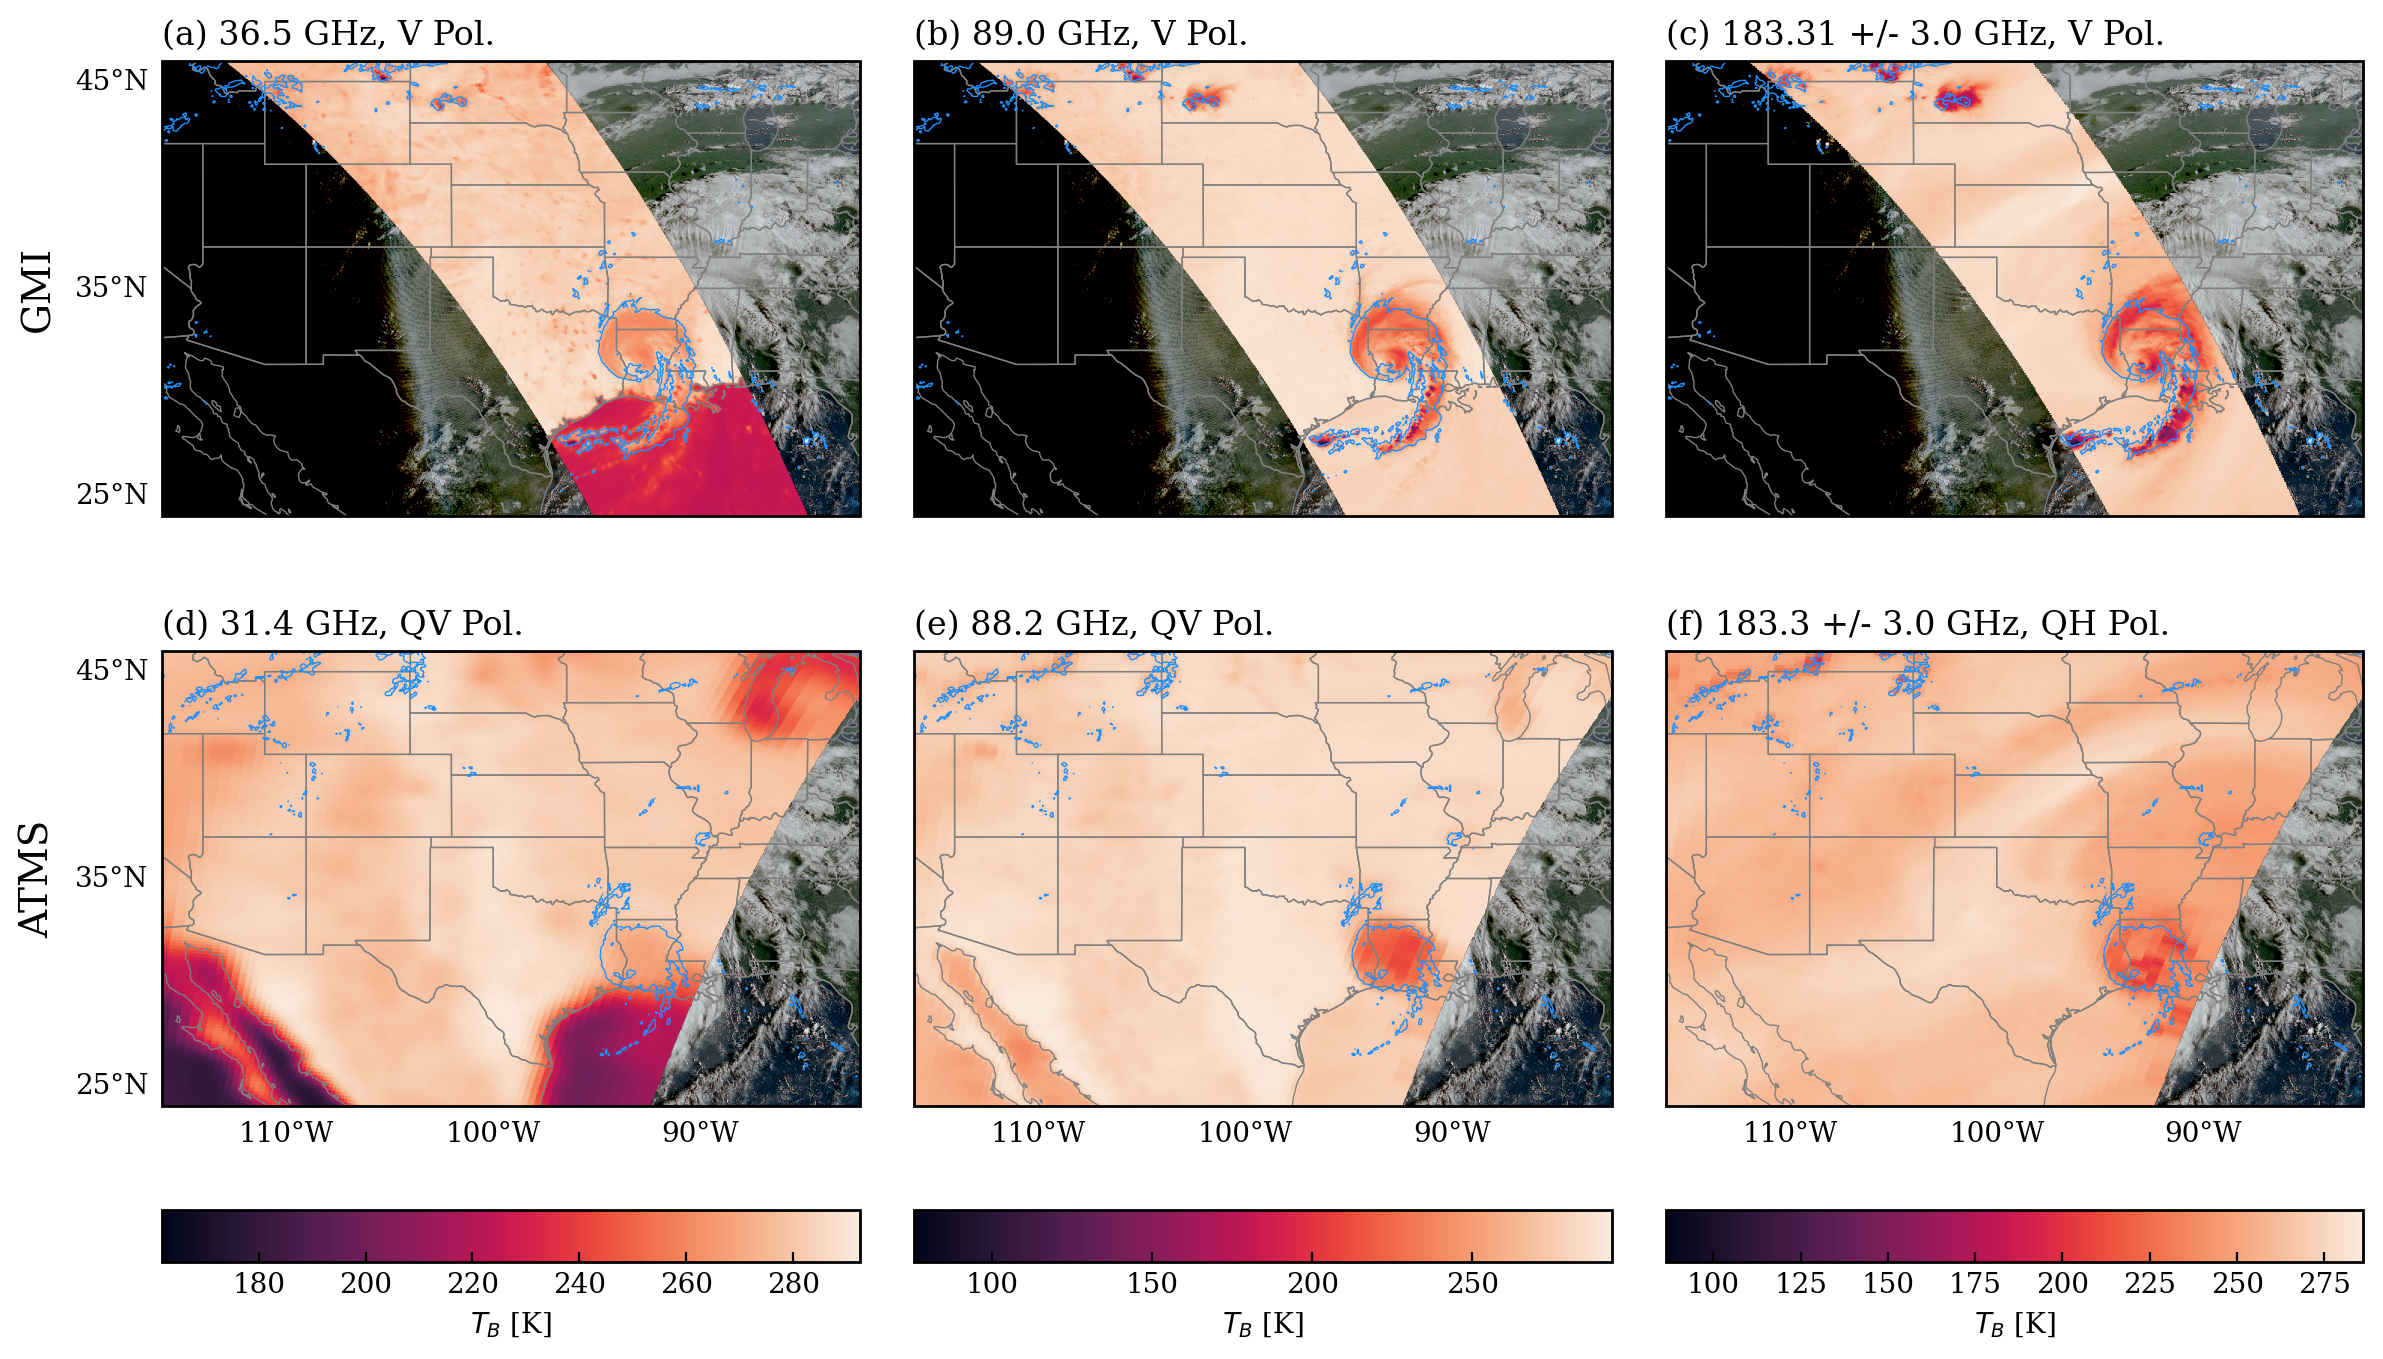
\includegraphics[width=1.0\textwidth]{figures/fig02}
	\caption{
		Passive microwave observations from the GMI (a - c) and ATMS (d - f)
		sensors during landfall of Hurricane Laura on August 27, 2020. The top
		row displays three selected channels from the GMI sensor, highlighting
		its high-resolution but limited swath. The bottom row presents
		corresponding channels from the ATMS sensor for comparison. The blue
		contour line encloses regions with surface precipitation rates exceeding
		1 mm h$^{-1}$.
	}
	\label{fig:observations_pmw}
\end{figure}

The PMW observations used to build the SatRain dataset are sourced from two
different sensors: the GPM Microwave Imager (GMI, \citeauthor{Draper2015GMI},
\citeyear{Draper2015GMI}) aboard the GPM Core Observatory, and a selection of
channels of the Advanced Technology Microwave Sounder (ATMS,
\citeauthor{Goldberg2006ATMS}, \citeyear{Goldberg2006ATMS}) aboard the Suomi
National Polar-orbiting Partnership satellite. The channels included from each
sensor are listed in Table 1. The GMI and ATMS sensors were chosen to represent
two ends of the spectrum of PMW instrumentation used for measuring
precipitation. GMI, the flagship PMW sensor of the GPM constellation, has been
designed for precipitation remote sensing and features optimized spectral
coverage and comparably high spatial resolution. In contrast, ATMS was developed
primarily for operational weather forecasting and, compared to GMI, offers fewer
precipitation-sensitive channels and significantly coarser spatial resolution.

Figure~\ref{fig:observations_pmw} compares GMI and ATMS observations of
Hurricane Laura, collected at 12:41 UTC and 08:41 UTC, respectively, on August
27, 2020. GMI provides higher spatial resolution than ATMS, enabling it to
capture finer cloud and precipitation structures, but this comes at the expense
of swath width, which is considerably narrower and therefore limits spatial
coverage. The two instruments also employ different scanning strategies. GMI is
a conical scanner: its antenna beam sweeps out a cone relative to the
spacecraft, producing near-circular scanlines with nearly constant
Earth-incidence angle. This geometry ensures that polarization and viewing
characteristics remain consistent across the swath. ATMS, by contrast, uses a
cross-track scanning approach. Here, footprint size increases away from nadir,
leading to reduced resolution toward the swath edges, while variations in
ray-path length and polarization angle introduce additional systematic
differences across the scan.

The PMW observations in SatRain are taken from the calibrated brightness temperature products of the GPM mission for GMI \citep{Berg2022_GMI_L1C_R_V07} and from ATMS aboard the NOAA-20 satellite \citep{Berg2022_ATMS_NOAA20_1C_V07}. The channels used in the dataset are summarized in Table~\ref{tab:pmw_channels}, along with their polarizations and approximate footprint sizes. Because the GPM data product does not include the ATMS temperature-sounding channels near \SI{50}{\giga\hertz}, these channels are likewise excluded from the SatRain ATMS subset.

\begin{table}[htbp]
	\centering
	% === Left Table ===
	\begin{subtable}{0.45\textwidth}
		\centering
		\begin{tabular}{ccc}
			\multicolumn{3}{c}{GMI}            \\[0.5ex]
			\toprule
			Freq. [GHz] & Pol. & FP [km x km] \\
			\midrule
			10.65       & V    & 32 x 19       \\
			10.65       & H    & 32 x 19       \\
			18.7        & V    & 18 x 11       \\
			18.7        & H    & 18 x 11       \\
			23.8        & V    & 15 x 9.2      \\
			36.5        & V    & 14 x 8.6      \\
			36.5        & H    & 14 x 8.6      \\
			89.0        & V    & 7.2 x 4.4     \\
			89.0        & H    & 7.2 x 4.4     \\
			166.5       & V    & 7.2 x 4.4     \\
			166.5       & H    & 7.2 x 4.4     \\
			\bottomrule
		\end{tabular}
	\end{subtable}%
	\hfill%
	% === Right Table ===
	\begin{subtable}{0.45\textwidth}
		\centering
		\begin{tabular}{ccc}
			\multicolumn{2}{c}{ATMS}           \\[0.5ex]
			\toprule
			Freq. [GHz]       & Pol. & FP [km] \\
			\midrule
			23.800           & QV   & 75       \\
			31.400           & QV   & 75       \\
			88.2             & QV   & 32       \\
			165.5            & QH   & 16       \\
			183.31 $\pm$ 7.0 & QH   & 16       \\
			183.31 $\pm$ 4.5 & QH   & 16       \\
			183.31 $\pm$ 3.0 & QH   & 16       \\
			183.31 $\pm$ 1.8 & QH   & 16       \\
			183.31 $\pm$ 1.0 & QH   & 16       \\
			\bottomrule
		\end{tabular}
	\end{subtable}
	\caption{
	  Frequencies (Freq.), polarizations (Pol.), and footprint (FP) sizes of the
	  PMW observations included in the SatRain dataset. For GMI, footprint sizes are
	  reported as the full width at half maximum (FWHM) along and across the
	  boresight direction. For ATMS, only the nadir FWHM is given; at nadir the
	  footprint is circular and therefore represented by a single value. The
	  polarization of ATMS are denoted quasi-horizontal (QH) and quasi-vertical (QV)
	  as the polarization mixture changes with the earth-incidence angle.
	}
	\label{tab:pmw_channels}
\end{table}

\subsubsection{Geostationary Sensors}

\begin{figure}[htbp] % h=here, t=top, b=bottom, p=page of floats
	\centering
	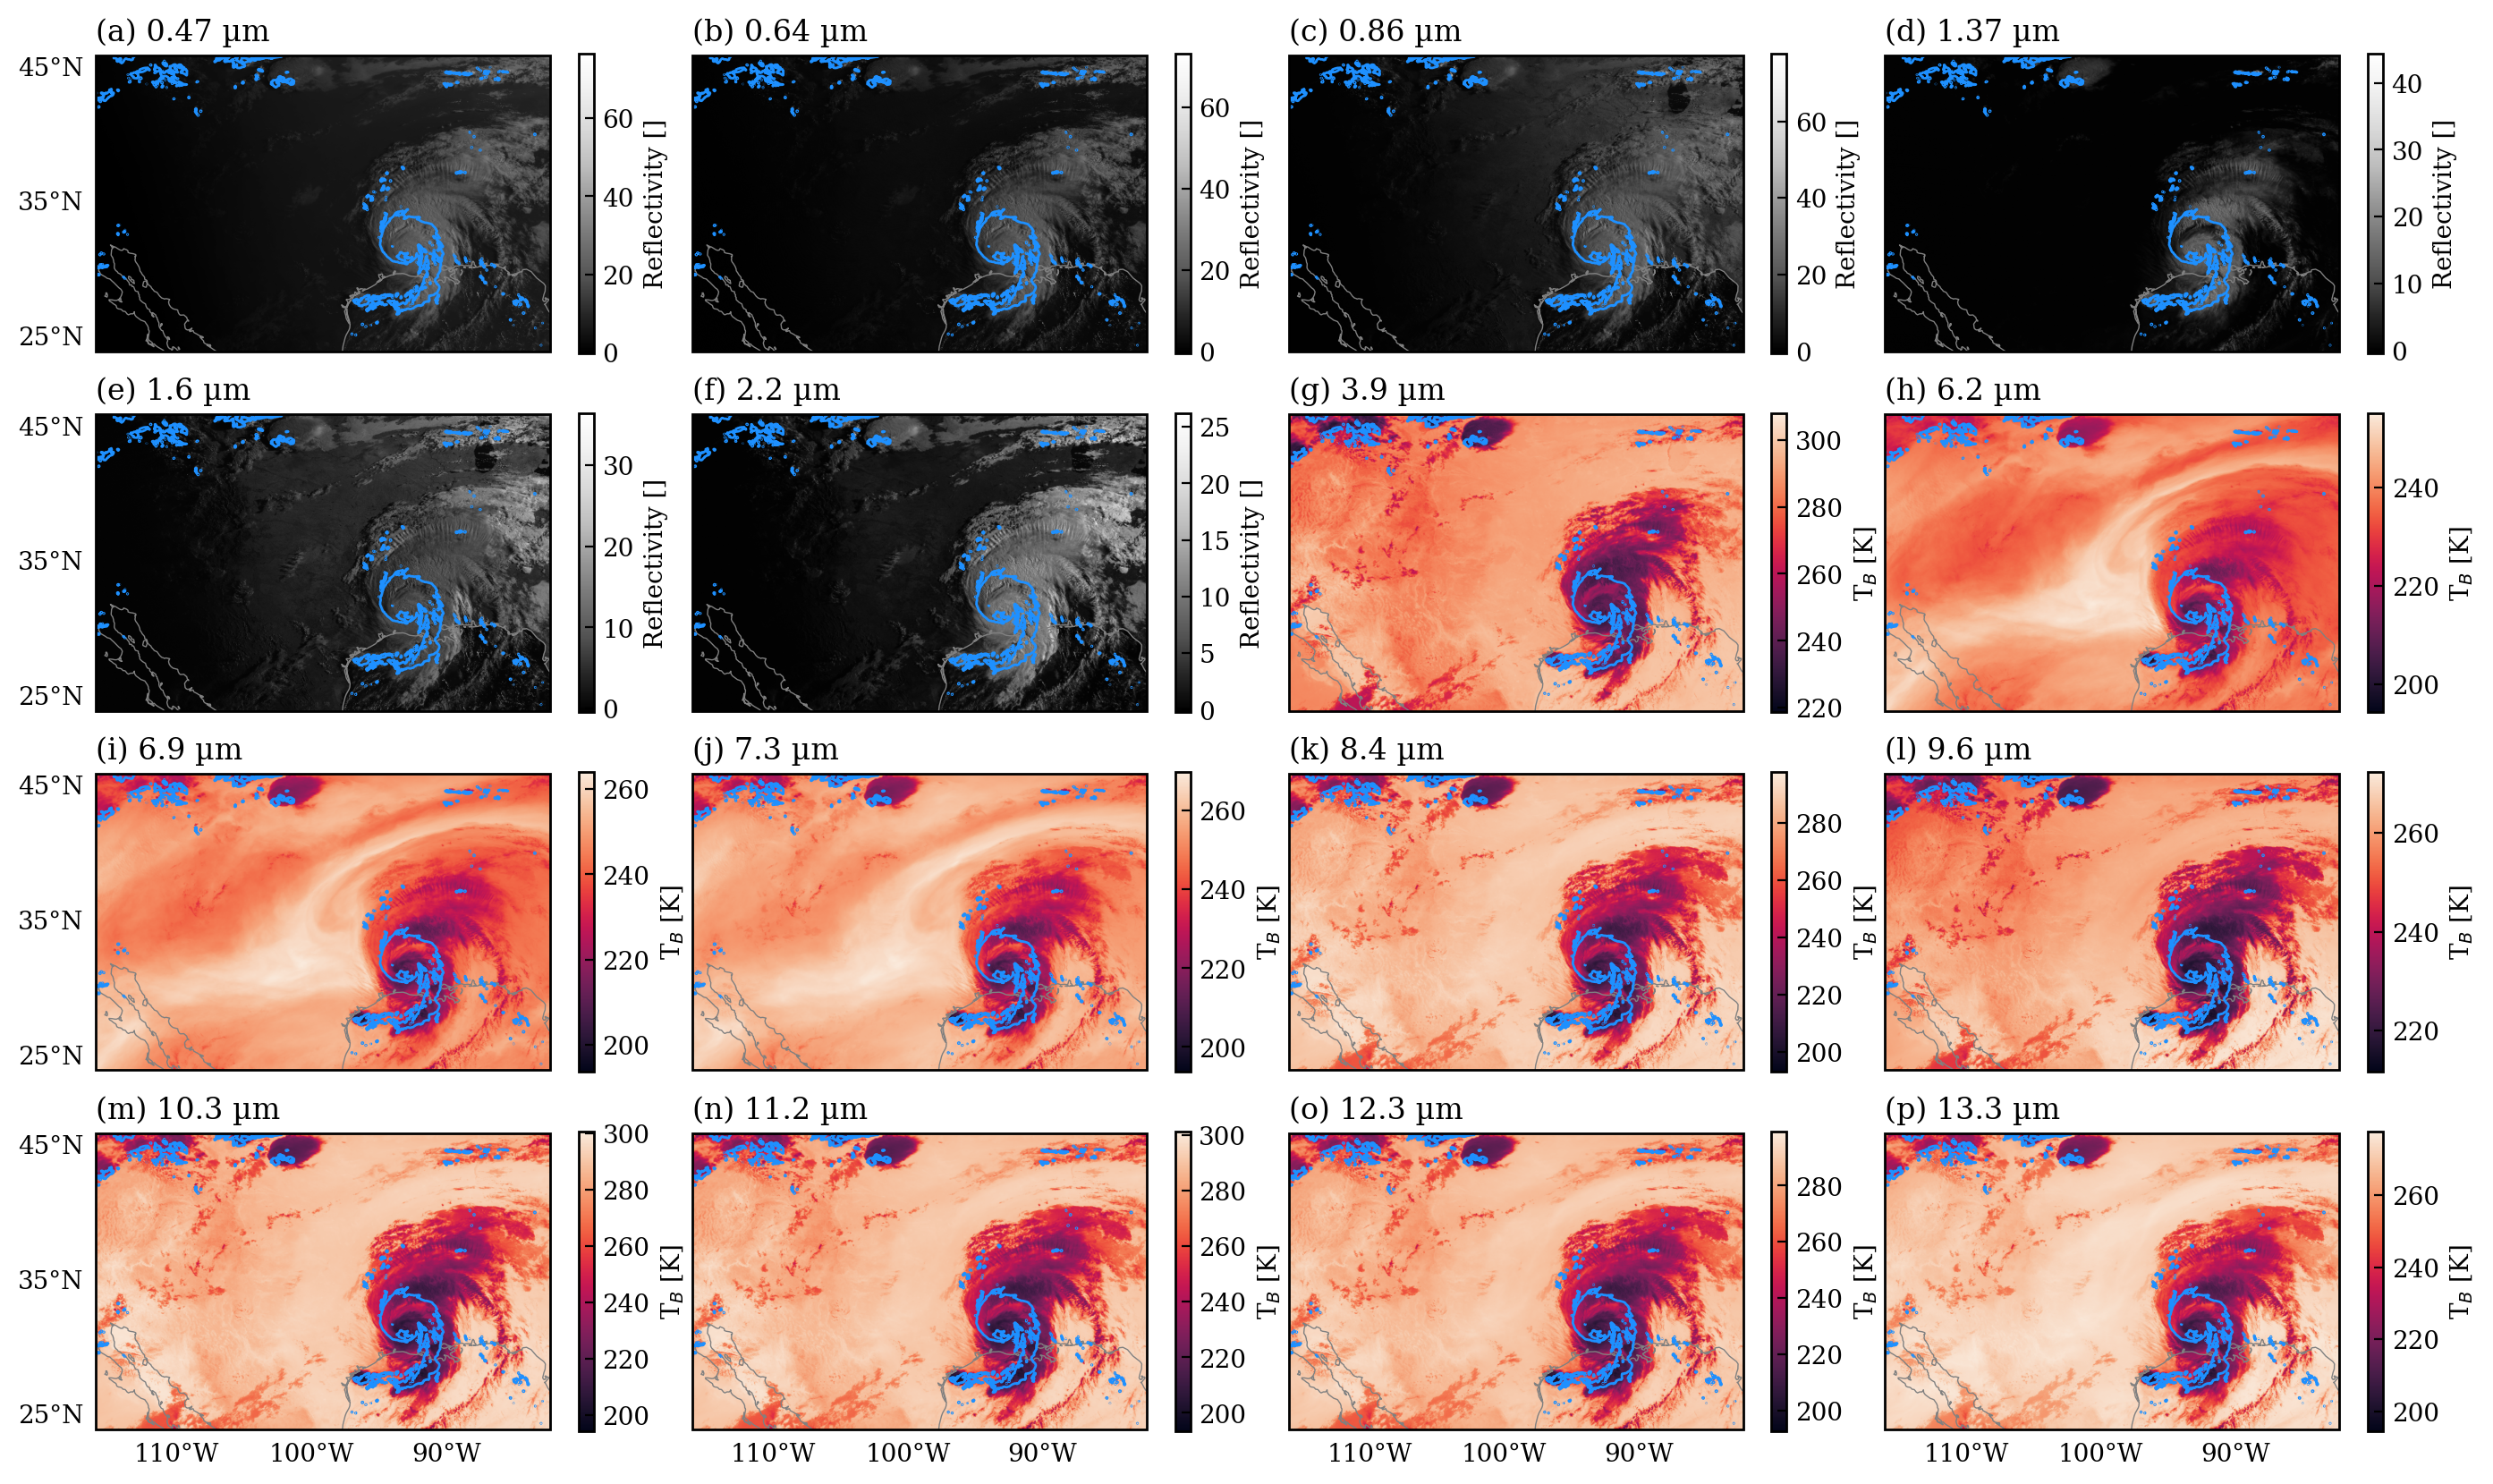
\includegraphics[width=1.0\textwidth]{figures/fig03}
	\caption{
		The 16 channels of the GOES ABI observing Hurricane Laura during
		landfall on August 27, 2020, at 08:41 UTC. The first six channels
		primarily measure reflected solar radiation. The remaining channels
		measure infrared radiation emitted from the atmosphere. Observations
		from geostationary sensors have the advantage of providing close-to
		continuous coverage but are sensitive primarily to cloud-top properties
		and thus only provide limited information on precipitation close to the
		surface. The blue contour encloses areas where surface precipitation
		exceeds \SI{1}{\milli \meter \per \hour}.
	}
	\label{fig:observations_geo}
\end{figure}


A principal limitation of passive microwave observations is their restricted
spatial and temporal coverage, as they are confined to the discrete overpass
times of low-Earth orbiting satellites. In contrast, visible (Vis) and infrared
(IR) sensors can achieve higher spatial resolutions due to the shorter
wavelength of the measured radiation allowing them to be deployed on
geostationary platforms. This allows for near-continuous monitoring of the
hemisphere below the satellite. As a result, geostationary observations are
essential for real-time and continuous precipitation monitoring.

Figure 3 shows observations from the 16 spectral channels of the Advanced
Baseline Imager aboard GOES-16 during the landfall of Hurricane Laura. The
native spatial resolution of ABI channels ranges from 500 meters to 2 kilometers
at the sub-satellite point on the equator. Although this resolution degrades
over the Continental United States due to increasing viewing angles, it remains
higher than that of PMW sensors. The first six channels are visible and
near-infrared bands that measure reflected solar radiation and are only
available during daylight hours. The remaining ten channels operate in the
thermal IR and provide data continuously, both day and night. Among the thermal
IR bands, the main distinguishing feature is their sensitivity to atmospheric
water vapor. For instance, channels centered at 6.2, 6.9, and \SI{7.3}{\micro
  \meter} are more sensitive to upper-tropospheric moisture and thus have
shallower penetration depths. This sensitivity to water vapor provides
contextual information on the moisture content of the air.

A particular challenge related to incorporating geostationary observations into
global precipitation retrievals is that the channels availability changes
between platforms and thus the geographical coverage regions. SatRain integrates
data from CONUS, the Korean peninsula, and Austria, which are covered by
different geostationary platforms. While observations over CONUS are derived
from the GOES 16 \citep{Goodman2019GOESR} platform, observations over Korea are
derived from the Himawari 8 and 9 platforms \citep{Bessho2016Himawari}, and
observations over Austria from the Meteosat 10 platform
\citep{Schmetz2002Introduction}. Table~\ref{tab:geo_channels} lists the central
wavelengths and corresponding bandwidths for the channels included from the ABI
sensor on GOES 16, the Advanced Himaware Imager (AHI,
\citeauthor{Da2015Preliminary}, \citeyear{Da2015Preliminary}), and the SEVIRI
\citep{Aminou2002Msg} sensor on Meteosat 10. The observations from the ABI, AHI,
and SEVIRI sensors were downloaded from \cite{NOAA_GOES_AWS},
\cite{NOAA_HIMAWARI_AWS}, and \cite{EUMETSAT_SEVIRI}.

\begin{table}[htbp]
  \centering
    \begin{tabular}{lccc}
      \toprule
      Channel & ABI & AHI & SEVIRI \\
      \midrule
      1 & 0.47 & 0.455 & 0.75  \\
      2 & 0.64 & 0.51  & 0.635 \\
      3 & 0.86 & 0.645 & 0.81  \\
      4 & 1.38 & 0.86  & 1.64  \\
      5 & 1.61 & 1.61  & 3.92  \\
      6 & 2.26 & 2.26  & 6.25  \\
      7 & 3.9  & 3.85  & 7.35  \\
      8 & 6.15 & 6.25  & 8.7   \\
      9 & 7.0  & 6.95  & 9.66  \\
      10 & 7.4  & 7.35  & 10.8 \\
      11 & 8.5  & 8.6   & 12.0 \\
      12 & 9.7  & 9.63  & 13.4 \\
      13 & 10.3 & 10.45 & 13.7 \\
      14 & 11.2 & 11.20 &    \\
      15 & 12.3 & 12.35 &    \\
      16 & 13.3 & 13.3  &    \\
      \bottomrule
	\end{tabular}
	\caption{Channel central wavelengths ABI sensor on GOES-16, the AHI sensor on Himawari-8/9, and the SEVIRI sensor on Meteosat-10.}
\end{table}

Latest-generation geostationary platforms provide observations at temporal
resolution of at least 10 minutes allowing them to closely track the evolution of
precipitation systems. In order to allow users to explore the temporal
information content in time-resolved geostationary observations, the SatRain
dataset includes observations from multiple time steps around the overpass of
the PMW sensor.

In addition to the multi-channel Vis and IR observations from the latest
generation of geostationary sensors, the SatRain dataset also integrates
0.036-degree gridded thermal IR observations from the \SI{11}{\micro \meter}
infrared window sourced from the Climate Prediction Center (CPC) global gridded
geostationary IR dataset \citep{NCEP_CPC_L3_IR}. Since these observations are
available almost continuously from 1998, they play an important role for
generating long-term precipitation records and are included as an independent
input data source in the SatRain dataset.


\subsubsection{Ancillary Data}

\begin{figure}[htbp] % h=here, t=top, b=bottom, p=page of floats
	\centering
	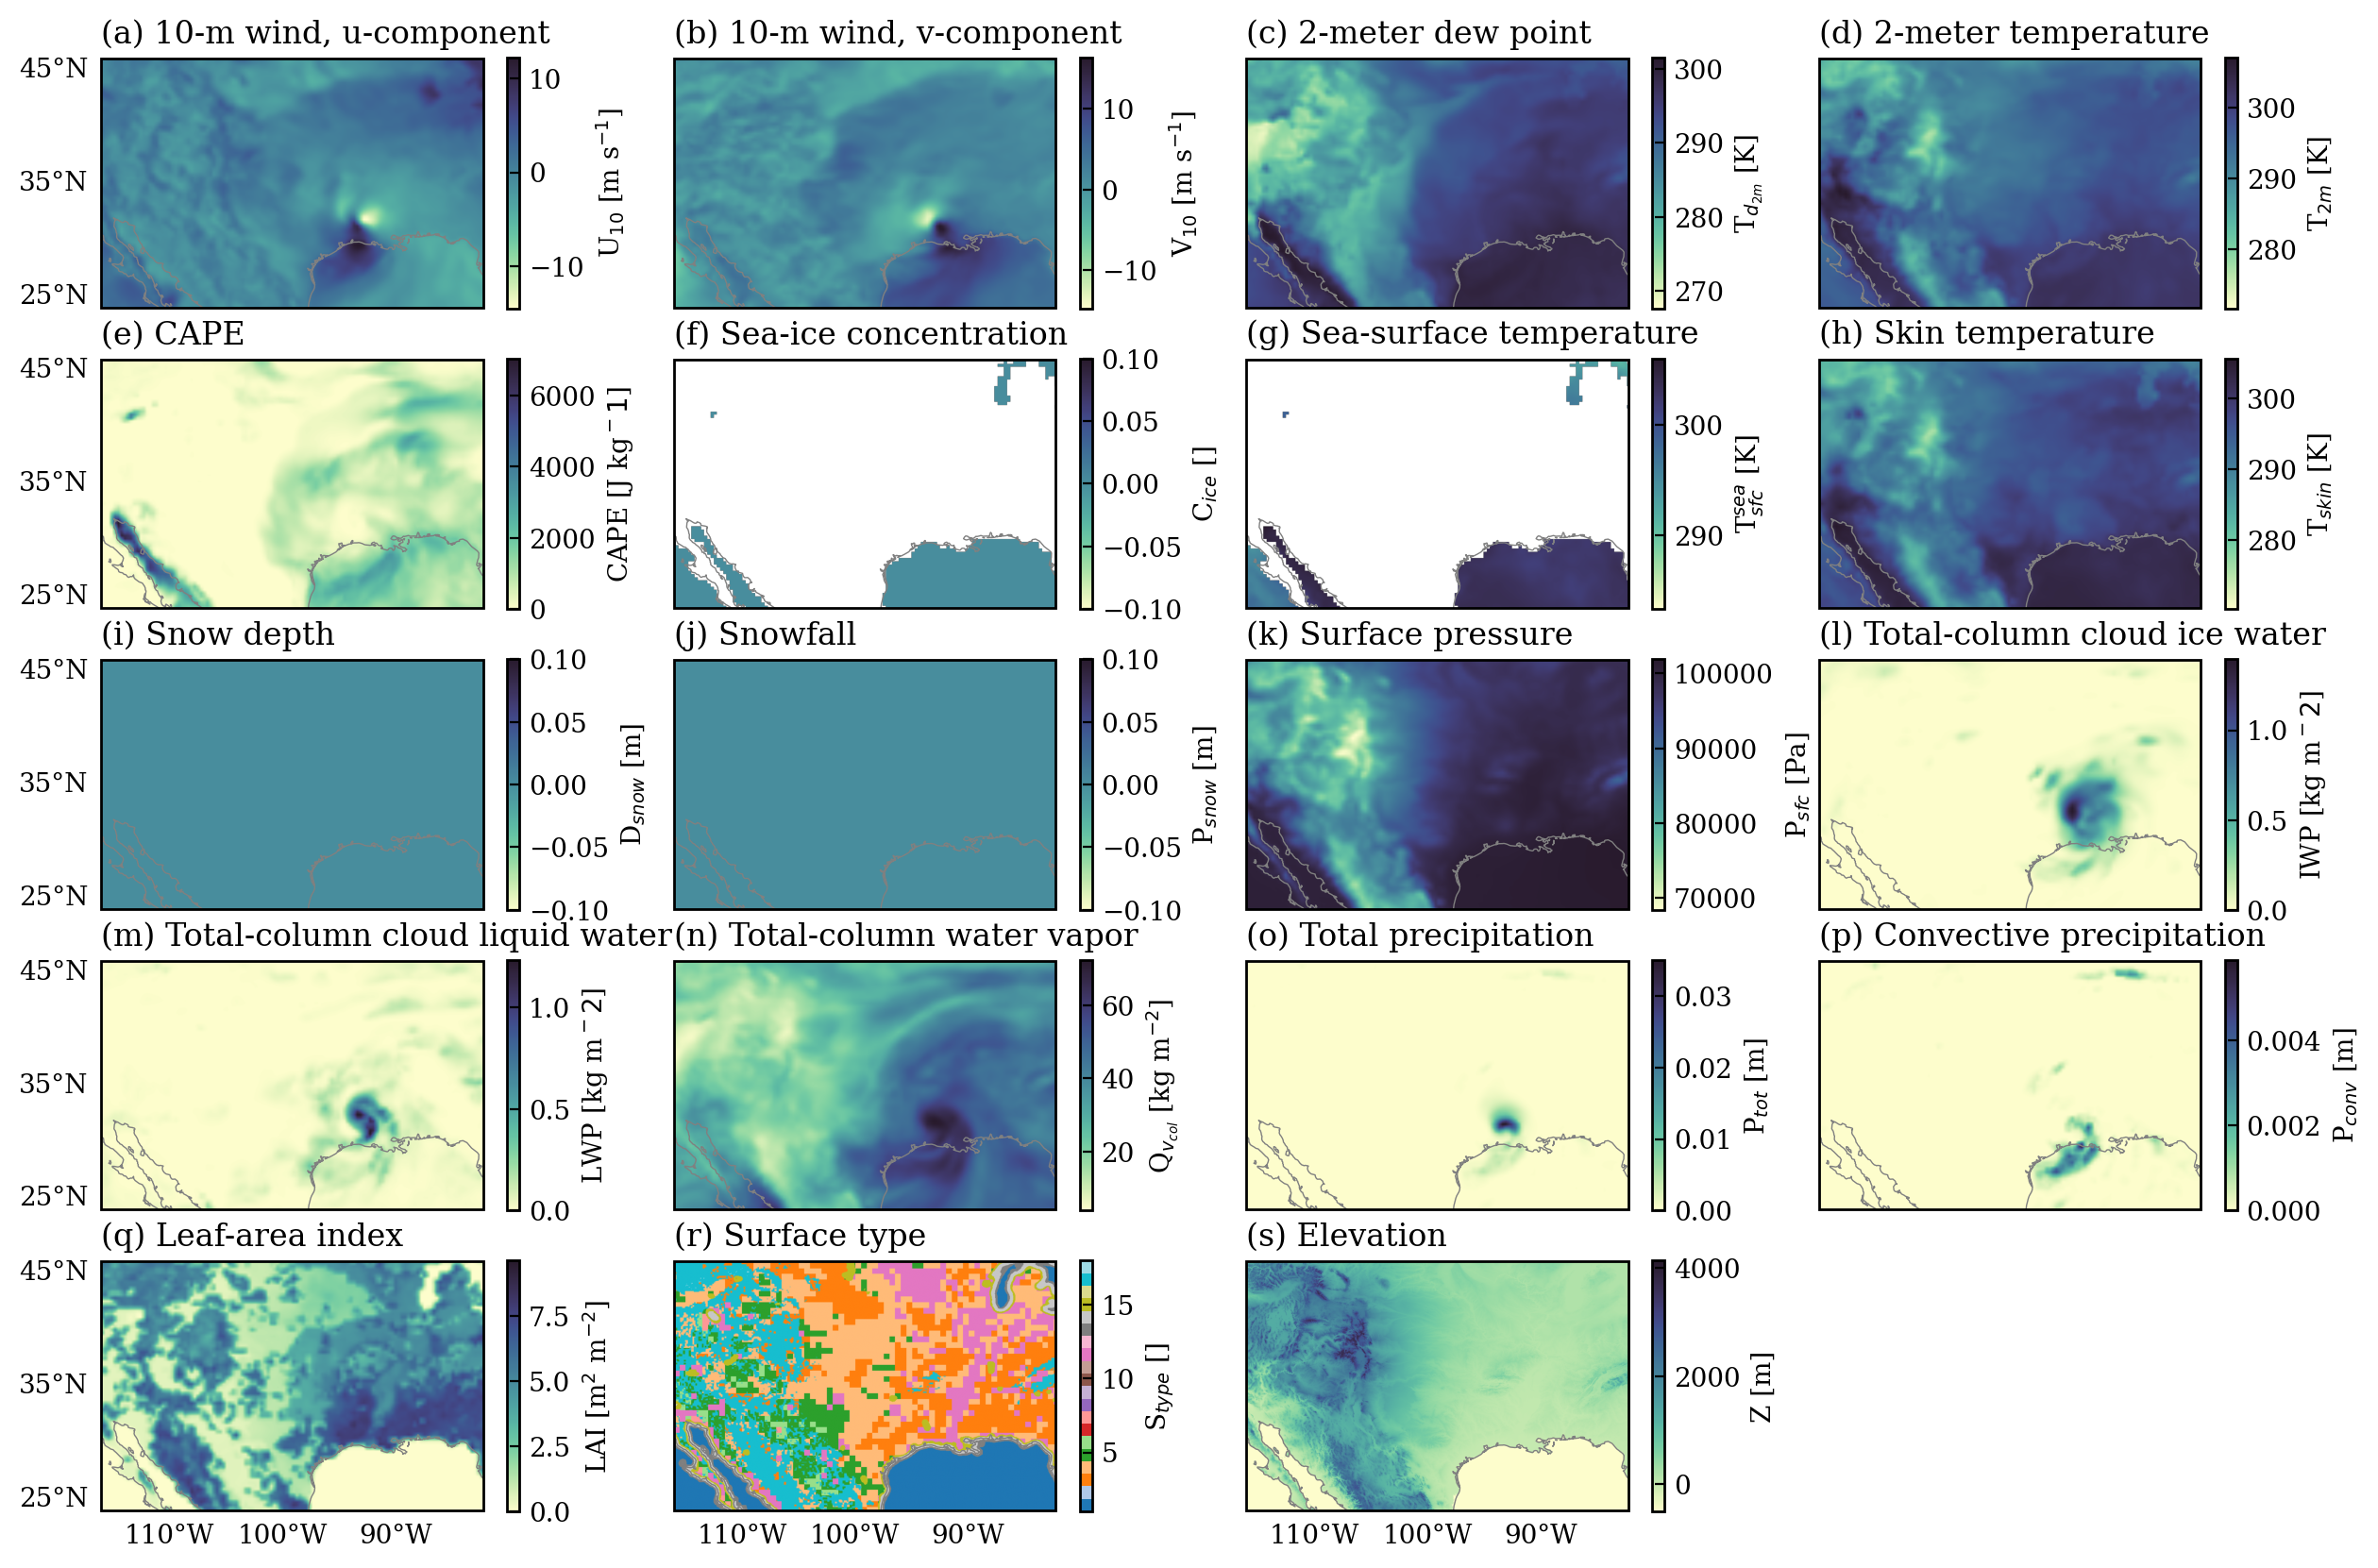
\includegraphics[width=1.0\textwidth]{figures/fig04}
	\caption{
		Ancillary variables provided by the SatRain dataset for the scene
		depicted in Fig. 1. Panels (a) to (q) show the dynamic ERA5 fields included in
		the ancillary data. Panel (r ) shows the 18-class surface classification from
		the GPROF algorithm and panel (s) the surface elevation from the NOAA Globe
		dataset.
	}
	\label{fig:ancillary_data}
\end{figure}

Because the relationship between satellite observations and surface
precipitation is often under-constrained, it is common to augment satellite
observations with complementary environmental information, so-called ancillary
data, to improve the accuracy of the precipitation estimates. Typical examples
include the surface type, atmospheric and surface temperatures, humidity, and
elevation. The SatRain dataset includes several static and dynamic ancillary
variables. Dynamic ancillary data describing the state of the atmosphere and the
surface are derived from the ERA5 \citep{Hersbach2020ERA5} dataset. In addition
to that, the ancillary data also contains an 18-class surface classification
that has been developed for the Goddard Profiling Algorithm (GPROF,
\citeauthor{GPM_GPROF_ATBD_V7}, \citeyear{GPM_GPROF_ATBD_V7}) precipitation
retrieval and combines microwave-based surface-type information with snow- and
sea-ice coverage data from the Autosnow product \citep{NCEI2025SNOWMaps}. In
terms of static variables, SatRain provides the surface elevation sourced from
the NOAA Global Land One-kilometer Base Elevation (GLOBE) digital elevation
model \citep{Hastings1999GLOBE}. Figure~\ref{fig:ancillary_data} provides
showcases the ancillary variables included in the SatRain dataset for the
landfall of Hurricane Laura.

\subsubsection{Precipitation Reference}

\begin{figure}[htbp] % h=here, t=top, b=bottom, p=page of floats
	\centering
	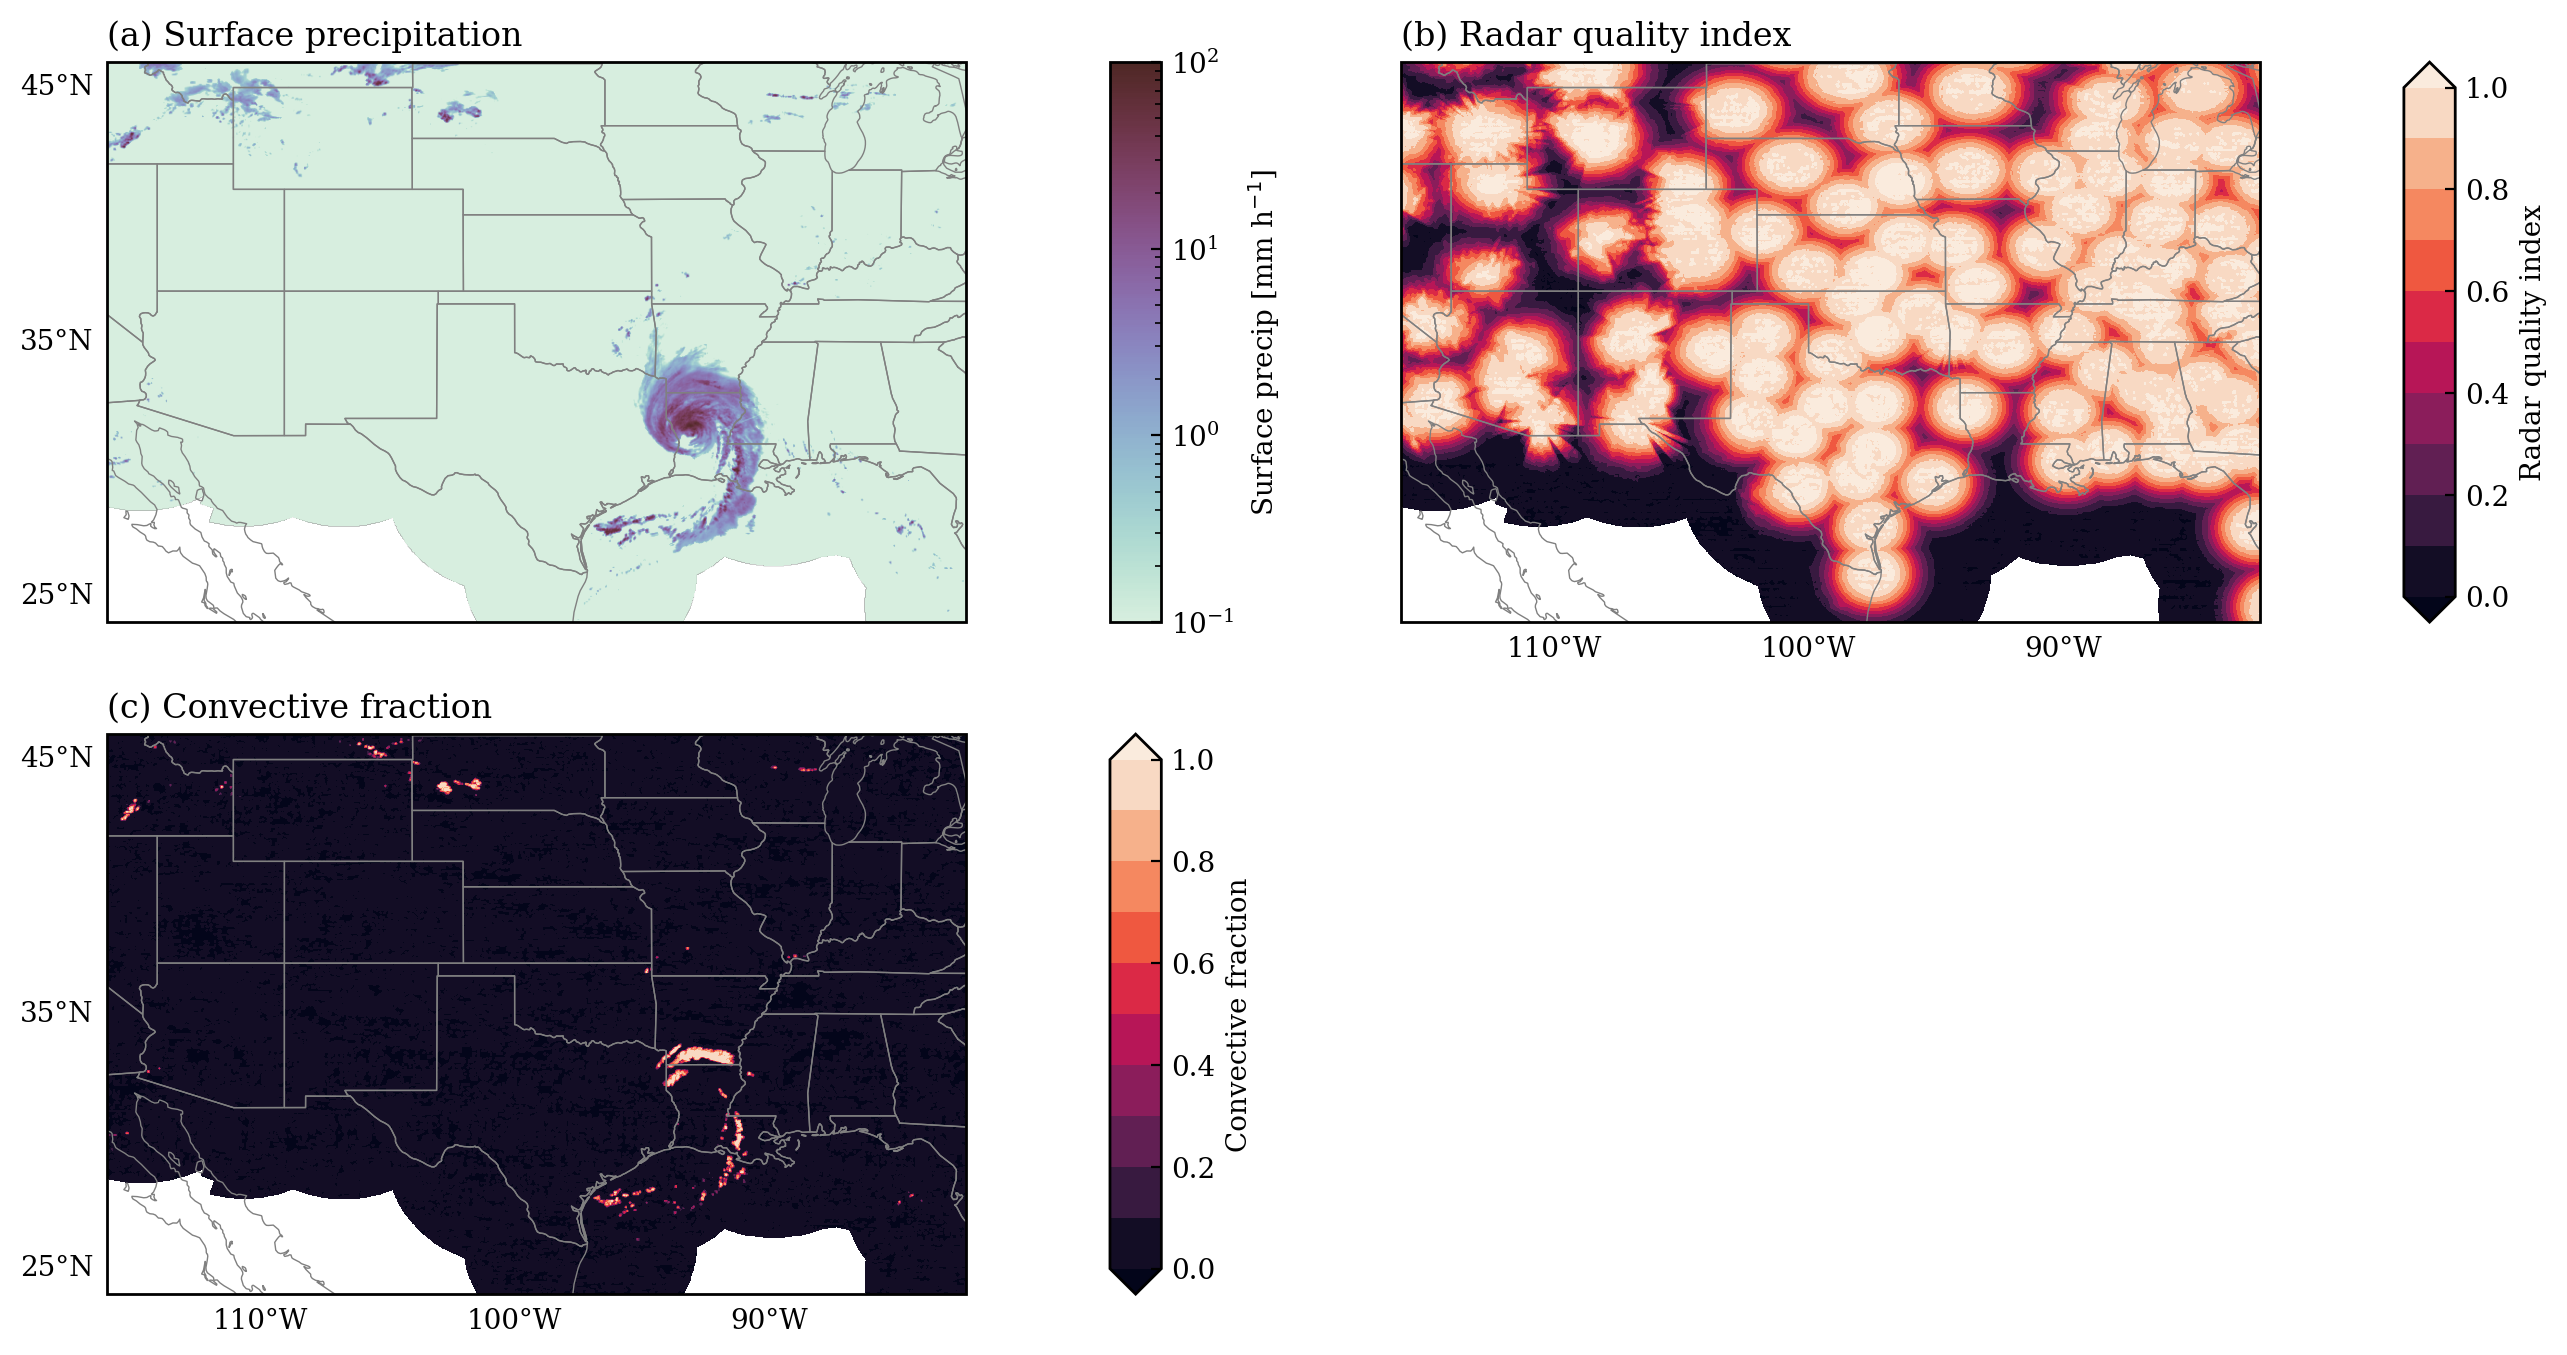
\includegraphics[width=1.0\textwidth]{figures/fig05}
	\caption{
		Reference precipitation estimates and auxiliary fields dataset during
		the landfall of Hurricane Laura. Panel (a) shows surface precipitation
		estimates from NOAA’s gauge-corrected Multi-Radar Multi-Sensor product.
		Panel (b) displays the radar quality index quantifying the reliability
		of the precipitation estimates. Panel (c) presents the convective
		fraction field, illustrating the hydrometeor classification data
		included in the SatRain dataset.
	}
	\label{fig:observations_geo}
\end{figure}

The precipitation reference used in the SatRain dataset are derived from
gauge-corrected ground-based precipitation radar measurements from NOAAs
gauge-corrected Multi-Radar Multi-Sensor (MRMS, \citeauthor{Smith2016MRMS},
\citeyear{Smith2016MRMS}) product. MRMS is based on radar observations from
Nexrad, the most extensive network of precipitation radars in the world
comprising around 160 polarimetric S-band radars. The radar-derived estimates of
liquid precipitation are corrected using hourly gauge-correction factors thus
enforcing consistency between instantaneous estimates and direct measurements of
hourly accumulations from gauge stations. While a certain level of residual
uncertainty in these estimates cannot be eliminated, they are generally
considered to be the best currently available estimates of surface precipitation
with near-complete coverage over CONUS. In addition to reference surface
precipitation rates, the SatRain dataset contains a radar quality index and the
gauge correction factor, allowing the user to customize the quality requirements
for the radar estimates used during both training and evaluation. Furthermore,
the dataset contains precipitation-type masks identifying convective and
stratiform rain, snow, and hail as provided by the MRMS data. Examples of these
fields are shown in Fig. 5.

\subsubsection{Independent Precipitation Reference}

\begin{figure}[htbp] % h=here, t=top, b=bottom, p=page of floats
	\centering
	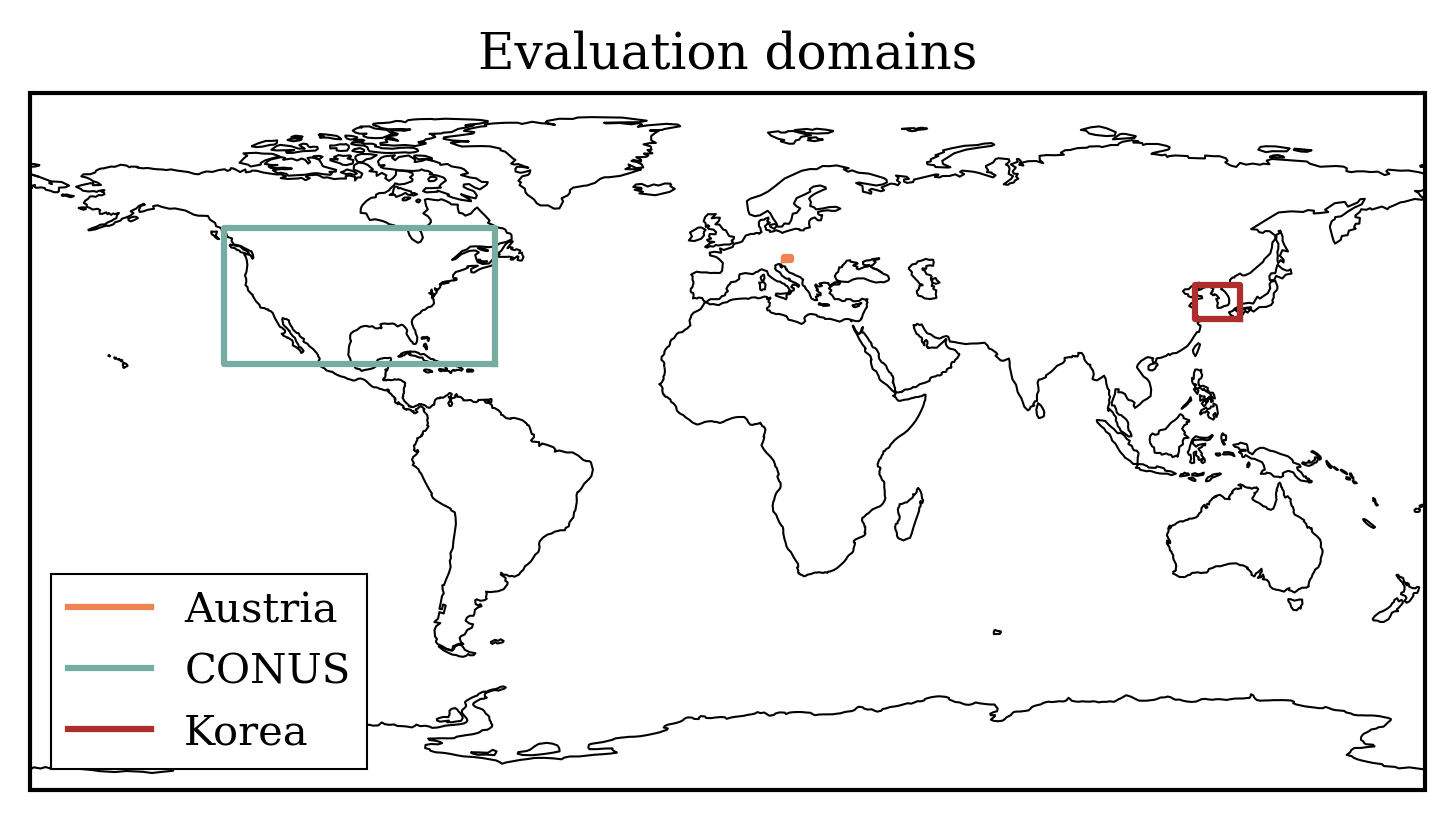
\includegraphics[width=1.0\textwidth]{figures/fig06}
	\caption{
		Independent test data included in the SatRain dataset. Panel (a) shows the
		spatial coverage of the three temporally and spatially independent test
		datasets. Panel (b) shows the location of the WegenerNet gauge stations used as
		reference measurements in the Austria domain and the grid they are aggregated
		to. Panel (c) shows an example in the Korea domain, with radar and rain-gauge
		data obtained from the Korea Meteorological Administration.
	}
	\label{fig:observations_geo}
\end{figure}


Since the SatRain training data is derived from four years (2019 - 2021) of ground-based radar measurements over CONUS, evaluating ML retrievals using this same data may lead to overfitting to specific weather patterns or measurement errors in the MRMS-based precipitation reference. To reduce the risk of overfitting on the weather patterns from the training period, the test data is derived from the year 2022. Moreover, the SatRain dataset includes two additional test datasets derived from different geographical regions and measurement systems.

The first geographically independent test dataset consists of gauge-corrected,
ground-based radar rainfall estimates over South Korea, generated using radar
compositing methods optimized for the Korean domain
\citep{Kwon2015RadarComparison}. The Korea-specific merging technique uses
radial basis function interpolation to combine radar and rain gauge observations
resulting in a high-resolution rainfall product in both space and time \citep{Ryu2025RBFMerging}.
Although the measurement approach is similar to that used in the MRMS reference
data over CONUS, the processing of raw data into precipitation estimates
differs. The dataset also represents a distinct climate regime from the training
data, offering a valuable test of the precipitation retrieval model’s ability to
generalize beyond the conditions typically encountered over CONUS. Studies such
as \cite{Sohn2013WarmRain} showed that cloud characteristics affecting both PMW
radiometers and IR observations differ substantially between Korea and CONUS and
can cause significant biases in algorithms applied to these two regions. The
independent testing data from Korea thus provides an opportunity to assess
whether retrieval improvements are achieved at the cost of global
generalizability.

The second independent evaluation dataset is derived from gauge measurements from the WegenerNet \citep{Fuchsberger2021WegenerNet} gauge network around the Feldbach region in Austria. While IPWG focuses primarily on gauge-corrected radar data for validation, WegenerNet is unique in that its gauge density is sufficiently high that the addition of radar data would not modify any of the gauge accumulations. In addition, it offers validation over a mountainous regime that radar/gauge networks still struggle with. For the comparison against satellite-based precipitation estimates the measurements from the ground stations were aggregated to the 0.036-degree grid using binning. As can be seen in Panel (b) of Fig. 6, the gauge density is sufficient to cover 24 grid cells with at least two gauges per cell. The mapping of the gridded measurements to the on-swath geometry was performed using nearest-neighbor interpolation.


\subsection{Dataset Generation}

In contrast to observations from geostationary sensors and ground-based reference data, passive microwave observations from GMI and ATMS are available only at discrete overpass times. The SatRain dataset is generated by extracting observations from all available overpasses of the GMI and ATMS sensor during the time period January 2018 to January 2023 and adding the corresponding geostationary observations, ancillary data, and ground-based reference precipitation estimates. The resulting collocation scenes are then used to extract fixed-size training scenes that can be used to train both pixel-based as well as scene-based ML-based precipitation estimation and detection models.

The training, validation, and testing splits of the SatRain dataset are chosen so that they are always either temporally or spatially independent. The training and validation data are extracted from the years 2019 up and including 2021. Data from the five first days of every month are assigned to the validation set and data from the remaining days to the training data set. The CONUS testing data is derived from the year 2022. The independent testing data over Austria uses observations from the years 2021 and 2022. The independent testing data over Korea uses observations from October 2022 to October 2023.

\subsubsection{Generation of Collocation Scenes}

\begin{figure}[htbp]
	\centering
	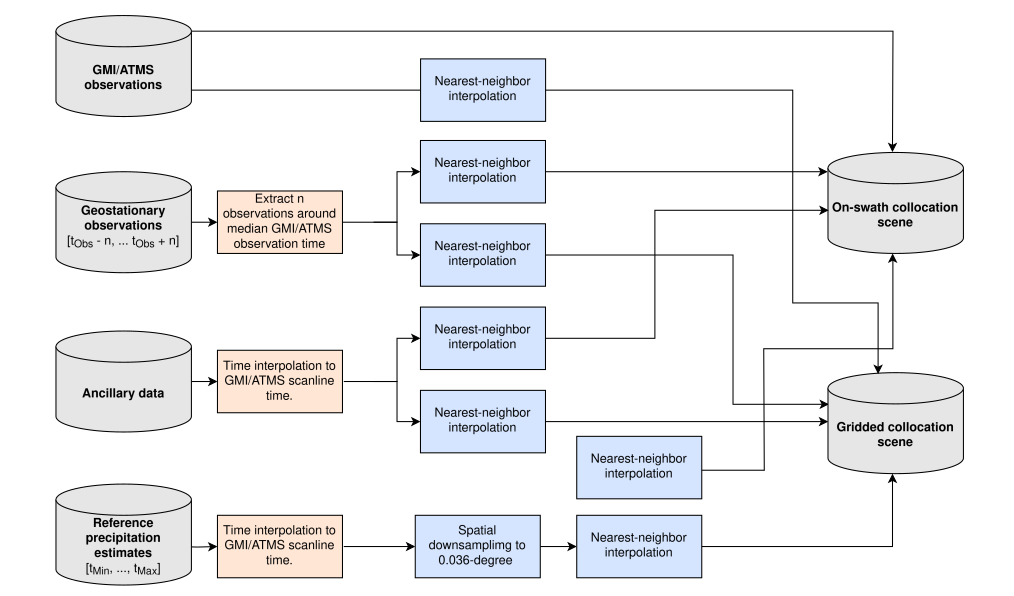
\includegraphics[width=1.0\textwidth]{figures/fig07}
	\caption{
		Flow diagram illustrating the data flow for collocating the satellite
		observations and ground-based reference precipitation estimates for the SatRain
		dataset.
	}
	\label{fig:data_flow}
\end{figure}

The first step of the generation of the SatRain dataset is the generation of
collocation scenes for every overpass of the PMW base sensor, i.e., GMI or ATMS,
over the targeted domain. The resulting collocation scene contains all retrieval
input data, i.e. satellite observations and ancillary data, combined with the
coincident reference precipitation on a common spatial grid. Two collocation
scenes are extracted for every overpass of the base sensors: An on-swath scene,
which uses the native sampling of the PMW observations, and a gridded scene,
which contains all data regridded to a regular latitude-longitude grid with a
resolution of 0.036 degree.

The collocation process, as illustrated in Figure~\ref{fig:data_flow}, starts
out with the PMW observation from an overpass of GMI or ATMS over the domain
containing the reference data. Corresponding ground-based reference data and
ancillary data are extracted to cover the time range of the overpass and
interpolated to the observation time of each scan-line of the PMW observations.
The MRMS data, which have a native resolution of 0.01 degree, are reduced in
resolution to match 0.036-degree grid by smoothing using a Gaussian filter with
a full width at half maximum of 0.036 degrees and interpolated linearly to the
target grid. The mapping of the reference precipitation estimates to the
on-swath geometry is performed by nearest-neighbor interpolation. Similarly, the
PMW observations are mapped to the regular latitude-longitude grid by nearest
neighbor interpolation.

The global gridded IR geostationary observations are extracted over a time
window of 8 hours centered on the median overpass time at a temporal resolution
of 30 min. Multi-channel Vis and IR observations from the ABI, AHI, and SEVIRI
are extracted over a time window of 1 hour and a temporal resolution of 10
minutes. The Vis/IR observations are mapped to the gridded and on-swath
geometries using nearest-neighbor interpolation.

\subsubsection{Training Scene Extraction}

To generate AI-ready training and validation data from the collocation dataset,
fixed-size training scenes are extracted from the previously created collocation
dataset. Two separate sets of scenes are extracted for the gridded and on-swath
observation geometries. The scenes are extracted randomly, allowing an overlap
of up to 50\% between neighboring scenes, requiring 75\% of the pixels to
contain valid observations and reference data. The scene size for the gridded
data is 256 pixel $\times$ 256 pixels and 64 pixels $\times$ 64 pixels for the
on-swath data. The smaller size of 64 x 64 used for the on-swath data is due to
the limited width of the swaths of the PMW observations, which is 96 for ATMS
and 221 for GMI. The scene extraction process is illustrated in Fig. 7.


\begin{figure}[htbp] % h=here, t=top, b=bottom, p=page of floats
	\centering
	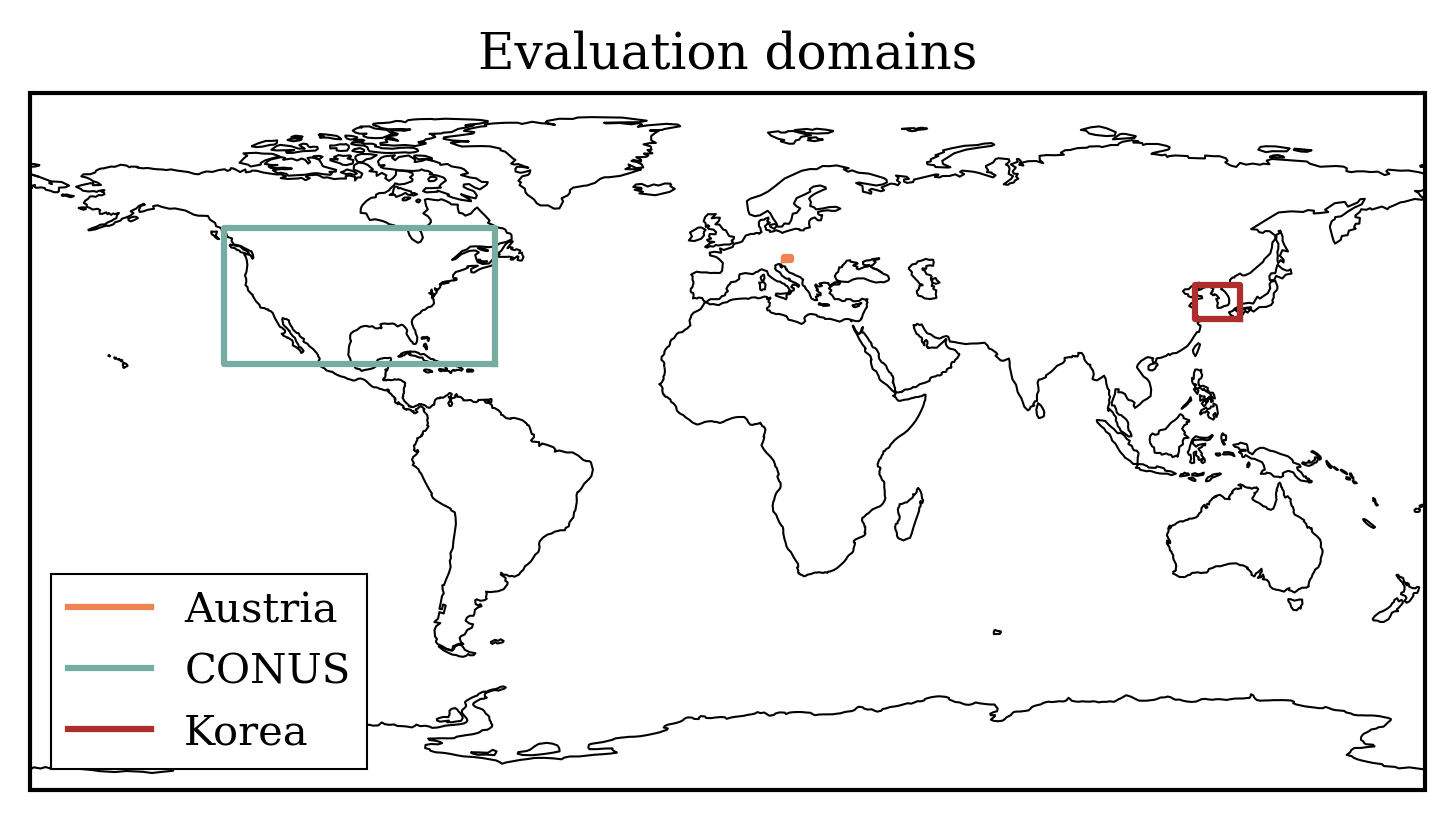
\includegraphics[width=1.0\textwidth]{figures/fig08}
	\caption{
		Fixed-size training scenes extracted from the SatRain collocation
		scenes. Panels (a), (b), and (c) show selected channels from the passive
		microwave (PMW), visible, and infrared observations that make up the
		input data of the SatRain dataset. Panel (d) shows the
		ground-radar-based precipitation reference used as training targets.
		Grey lines mark the outlines of the training samples extracted from this
		collocation scene for the gridded and on-swath observations. Black lines
		mark the sample training scenes displayed in Panel (e) and (f).
	}
	\label{fig:example_scenes}
\end{figure}


\section{Data Records}

\subsection{Dataset Organization}

The SatRain dataset consists of two independent subsets corresponding to collocations scenes extracted from GMI overpasses and ATMS observations, respectively. The underlying PMW sensor of each subset is referred to as the base sensor of the corresponding subset. For each base sensor, the data is split into training, validation, and testing splits following ML best practices. The training and validation splits share the same data format. The validation split contains samples from the first five days of each month and the training split the remaining data. While the validation set is generally intended for monitoring training progress, this is left to the user, who may also merge the two splits and use both for training.

The testing split is provided in both on-swath and gridded geometries but is not
divided into fixed-size scenes. Retaining the original observation structure
avoids sampling distortions and allows existing precipitation retrievals to be
evaluated directly on the test data.

The training and validation splits are split once more into subsets of different sizes: ‘xs’, ‘s’, ‘m’, ‘l’, and ‘xl’. This additional splitting of the data was performed to support users and compute systems with limited storage resources, while also providing a dataset large enough to train modern deep learning models.

The testing split is split into three spatial domains: ‘conus’, ‘korea’, ‘austria’, corresponding to the underlying reference data: MRMS over CONUS, ground-based radar data over Korea, and in-situ measurements from the WegenerNet stations in Austria.

\subsection{Data Files}

The various input and target data for each training scene are stored in separate
NetCDF4 files. This modular organization allows users to download just the data
they intend to use, for example, only the small ('\texttt{s}') subset of the GMI
and target data to train and evaluate a retrieval using only passive microwave
observations. Each file is identified using an individual prefix
('\texttt{gmi}', '\texttt{atms}', '\texttt{geo}', '\texttt{geo\_ir}',
'\texttt{ancillary}', '\texttt{target}') following a time stamp in the format
\texttt{YYYYMMDDHHMMSS} containing the median observation time. Input and target
files corresponding to a specific training, validation, or testing sample can
thus be identified using this timestamp.

Due to the large size of the time-resolved geostationary observations, the
geostationary observations are split into files containing only the observations
closest to the reference precipitation estimates and files containing
observations from multiple observations times. The multi-timestep observations
are stored in separate files with the suffix '\texttt{\_t}', i.e.,
'\texttt{geo\_t}' and '\texttt{geo\_ir\_t}'.

\subsubsection{PMW Observations}

The PMW observations in the SatRain dataset consist of observations from the GMI
sensor and the ATMS sensor on the NOAA-20 satellite. They are stored in files
labeled '\texttt{gmi\_\textlangle timestamp\textrangle.nc}' for the subset using
GMI as base sensor and, correspondingly, '\texttt{atms\_\textlangle
  timestamp\textrangle.nc}' for the subset using ATMS as base sensor. Each file
contains the brightness temperatures in Kelvin for each channel (\texttt{observations}), the
corresponding earth-incidence angles (\texttt{earth\_incidence\_angle}), and the observation time (\texttt{scan\_time}) corresponding to
each scan line. The channels included for the GMI and ATMS sensors are listed in
table~\ref{tab:pmw_channels}.

\subsection{Geostationary IR Observations}

The single-channel gridded IR observations from the global, merged CPC dataset
\citep{NCEP_CPC_L3_IR} are stored in files named '\texttt{geo\_ir\_\textlangle
  timestamp\textrangle.nc}' and contain IR window-channel observations from
  wavelengths around $\SI{11}{\micro \meter}$. The observed brightness
  temperatures in $\si{K}$ are stored in the variable \texttt{observations}. The
  single-timestep files contain the GEO IR observations closest to the
  measurement time of the reference precipitation estimates. The
  temporally-resolved GEO IR observations contain 16 half-hourly observations
  centered on the median observation time and are stored in files named
  '\texttt{geo\_ir\_t\_\textlangle timestamp\textrangle.nc}'.

\subsection{Geostationary Vis and IR Observations}

The multi-channel, geostationary Vis and IR observations are stored in files
named '\texttt{geo\_\textlangle timestamp\textrangle.nc}'. These files contain
  the observations closest in time to the measurement time of the reference
  precipitation estimates in the variable \texttt{observations}. The visible
  channels are stored as reflectances while thermal IR channels are stored using
  brightness temperatures. The geostationary data currently does not include
  viewing angles so the user will have to add them manually. The multi-timestep
  files (\texttt{geo\_t\_\textlangle timestamp \textrangle.nc}') contain
  observations from four 10-minute time steps prior to the collocation median
  and three 10-minute time steps after the collocation median time.

Since GOES observations are only available over CONUS, the geostationary
observations for the test data from the Korea and Austria domains are derived
from AHI sensor onboard Himawari 8 and 9 and the SEVIRI sensor onboard Meteosat
10. Table~\ref{tab:geo_channels} lists the central wavelengths of the
channels of each of the included sensors. Since the sensors have different
channels, the observations differ in their spectral coverage and users will need
to account for that in their algorithm design.

\subsection{Ancillary Data}

The ancillary data is stored in separate files named
'\texttt{ancillary\_\textlangle timestamp \textrangle.nc}'. Each file contains
  the ancillary variables listed in table~\ref{tab:ancillary}.

\begin{table}[htbp]
\centering
\begin{tabular}{lp{4cm}ll}
\toprule
\textbf{Variable name} & \textbf{Explanation} & \textbf{Unit} & \textbf{Source} \\
\midrule
\texttt{ten\_meter\_wind\_u} & Zonal wind at 10 m altitude & $\si{\meter \per \second}$ & ERA5 \\
\texttt{ten\_meter\_wind\_v} & Meridional wind at 10 m altitude & $\si{\meter \per \second}$ & ERA5 \\
\texttt{two\_meter\_dew\_point} & Dew-point temperature at 2 m altitude & $\si{\kelvin}$ & ERA5 \\
\texttt{two\_meter\_temperature} & Near-surface temperature & $\si{\kelvin}$ & ERA5 \\
\texttt{cape} & Convective available potential energy & $\si{\joule \per \kilo \gram}$ & ERA5 \\
\texttt{sea\_ice\_concentration} & Fractional sea-ice coverage & -- & ERA5 \\
\texttt{sea\_surface\_temperature} & Sea surface temperature & $\si{\kelvin}$ & ERA5 \\
\texttt{skin\_temperature} & Surface skin temperature & $\si{\kelvin}$ & ERA5 \\
\texttt{snow\_depth} & Snow depth & $\si{\kilo \gram \per \meter \squared}$ & ERA5 \\
\texttt{snow\_fall} & Snowfall rate & $\si{\meter \per \hour}$ & ERA5 \\
\texttt{surface\_pressure} & Surface pressure & $\si{\hecto \pascal}$ & ERA5 \\
\texttt{total\_column\_cloud\_ice\_water} & Vertically integrated mass of cloud ice & $\si{\kilo \gram \per \meter}$ & ERA5 \\
\texttt{total\_column\_cloud\_liquid\_water} & Vertically integrated mass of liquid cloud droplets & $\si{\kilo \gram \per \meter \squared}$ & ERA5 \\
\texttt{total\_column\_water\_vapor} & Vertically integrated mass of water vapor & $\si{\kilo \gram \per \meter \squared}$ & ERA5 \\
\texttt{total\_precipitation} & Total precipitation & $\si{\meter \per \hour}$ & ERA5 \\
\texttt{convective\_precipitation} & Convective precipitation & $\si{\meter \per \hour}$ & ERA5 \\
\texttt{leaf\_area\_index} & Half of the total green leaf area per unit ground area & \si{\meter \squared \per \meter \squared}$ & ERA5 \\
\texttt{surface\_type} & GPROF 18-class dynamic surface classification & -- & GPROF V7 \\
\texttt{elevation} & Surface elevation & $\si{\meter}$ & NOAA GLOBE \\
\bottomrule
\end{tabular}
\caption{List of the variables, their explanations, units, and data sources included in the ancillary data.}
\label{tab:ancillary}
\end{table}


\subsection{Reference Data}

The reference data for every scene is stored in a file
'\texttt{target\_\textlangle timestamp\textrangle.nc}', where the timestamp
matches that of the input data. The reference data files contain the surface
precipitation in a variable called '\texttt{surface\_precip}'. Additionally, the
reference data files derived over CONUS contain several quality indicator
variables that can be used to filter the reference data samples used for
training and validation. The primary quality indicator is the radar quality
index (\texttt{radar\_quality\_index}), which provides an estimate of the
quality of the surface precipitation estimates based on the radar beam height,
beam blockage, and the height of the freezing level. Moreover, the files contain
the gauge correction factor (\texttt{gauge\_correction\_factor}) that was
applied to correct the radar-only precipitation estimates. Finally, the files
also contain the fraction of valid (\texttt{valid\_fraction}), snowing
(\texttt{snow\_fraction}), and hailing (\texttt{hail\_fraction})
0.01-degree-resolution pixels within the downsampled 0.036 degree grid box of
the SatRain dataset. Since the radar data over Korea and the station data over
Austria do not provide this additional information, these auxiliary fields are
not provided by the target data files from the Korea and Austria domains.


\section{Technical Validation}

To demonstrate the practical value of the dataset as well as its technical
correctness, we have used the CONUS-based training data to train three different
precipitation retrievals using the three principal input-observations types,
i.e., multi-channel geostationary observations from the GOES ABI (GEO),
single-channel IR observations from the CPCIR dataset (GEO IR), and PMW
observations from GMI (GMI), and applied them to retrieve precipitation during
the landfall of Typhoon Khanun over Korea. The retrievals use satellite
observations only and do not make use of the ancillary data provided by the
SatRain dataset. The retrievals are implemented using a relatively shallow,
convolutional neural network with 10 million parameters. The resulting reference
and retrieved precipitation fields are compared to the reference ground-based
radar estimates, and two baselines from the ERA-5 reanalysis dataset and the
GPROF precipitation retrieval in Fig. 8.

\begin{figure}[htbp] % h=here, t=top, b=bottom, p=page of floats
	\centering
	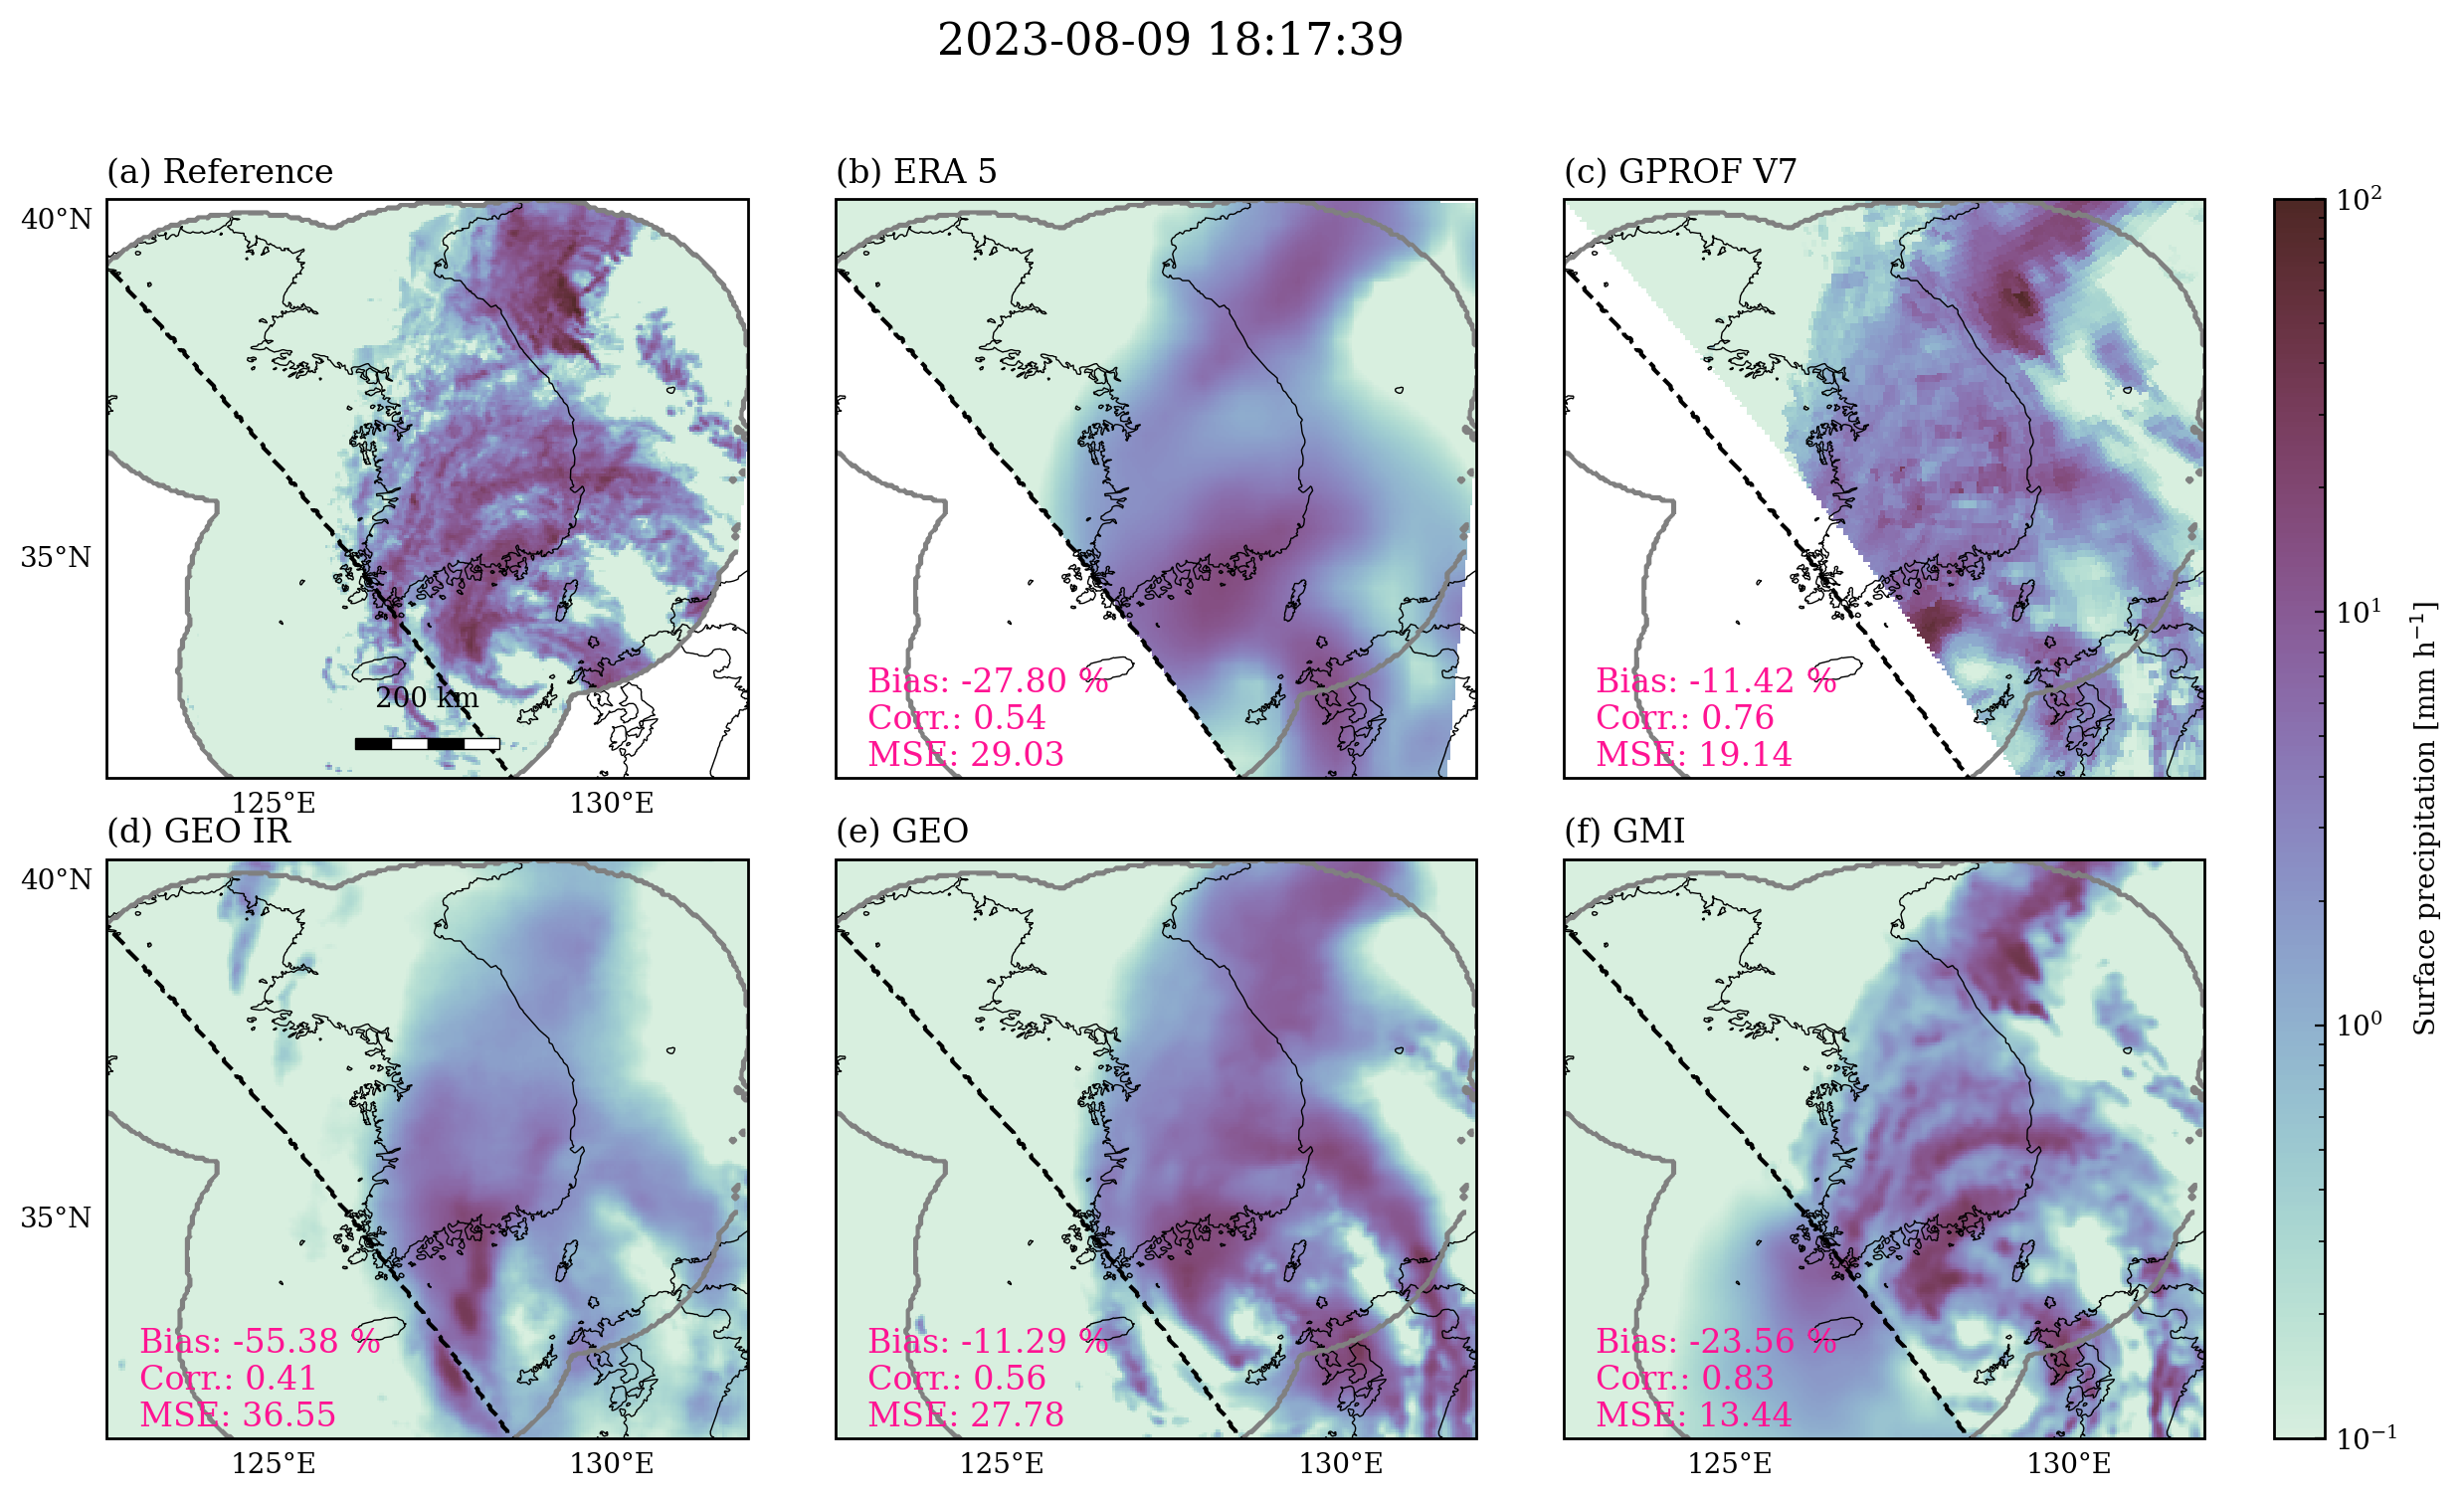
\includegraphics[width=1.0\textwidth]{figures/fig09}
	\caption{
	Precipitation retrievals trained using the CONUS-based SatRain
	training dataset compared to ground-based precipitation estimates and two
	baseline datasets during the landfall of Typhoon Khanun over the Korean
	peninsula. Panel (a) shows the ground-based reference precipitation
	estimates, panel (b) shows the precipitation field from the ERA5 reanalysis,
	panel (c) shows precipitation estimates from the GPROF precipitation
	retrieval applied to GMI observations. Panels (d), (e), and (f) show
	retrievals trained using the SatRain dataset over CONUS using multi-channel
	Vis/IR observation, single-channel GEO-IR observations, and GMI PMW
	observations, respectively.

	}
	\label{fig:case_study}
\end{figure}

The results demonstrate that all retrievals capture the main precipitation
structures of Typhoon Khanun, but with clear differences in accuracy reflecting
the information content of their input observations \citep{Kidd2011GPM}. The
PMW-based retrieval performs best, reproducing much of the fine-scale structure
evident in the reference estimates. The multi-channel geostationary retrieval
captures the primary precipitation bands but misses finer details resolved by
PMW. In contrast, the single-channel IR retrieval shows the weakest performance,
with limited structural detail and correspondingly lower linear correlation and
higher mean-squared error.

\begin{figure}[htbp] % h=here, t=top, b=bottom, p=page of floats
	\centering
	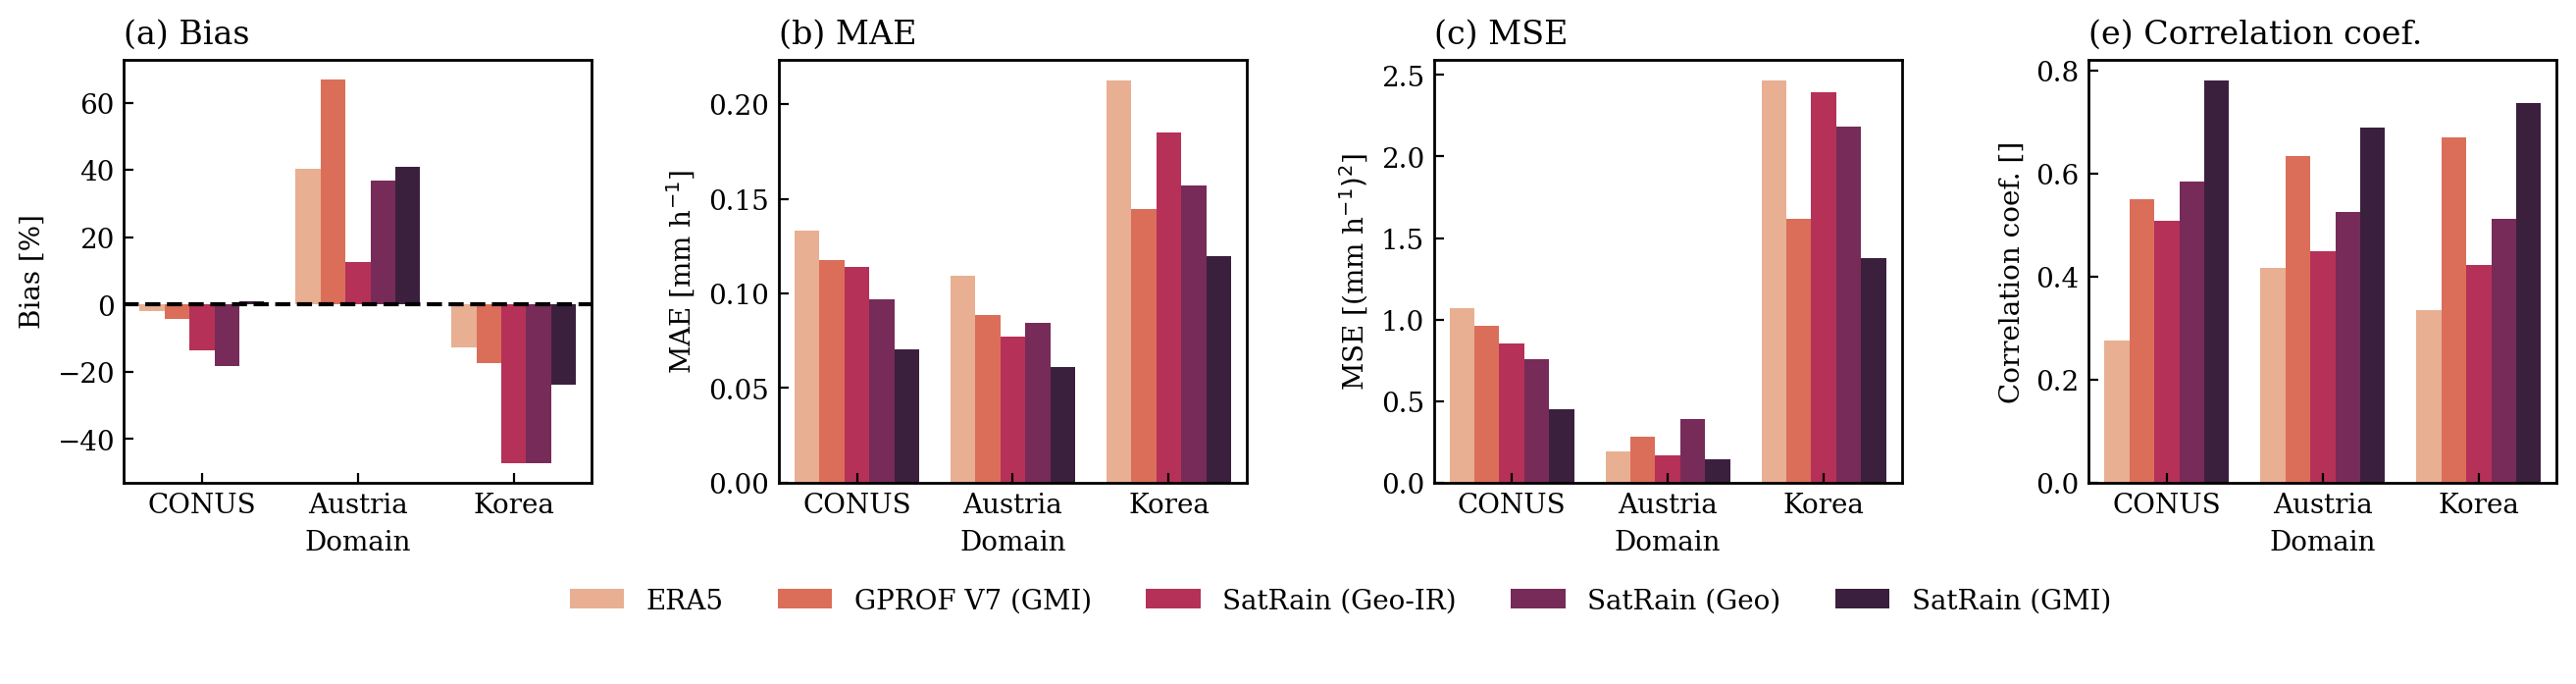
\includegraphics[width=1.0\textwidth]{figures/fig10}
	\caption{
	Evaluation of quantitative precipitation estimates from two state-of-the-art
	precipitation datasets (ERA5 and GPROF) and ML retrievals trained using the
	different satellite observations of the SatRain dataset. Each retrieval is
	evaluated for each of the three testing domains of the SatRain dataset. Panels
	(a) to (d) show the Bias, mean-absolute error (MAE), mean-squared error (MSE),
	and linear correlation coefficient, respectively.
	}
	\label{fig:sensor_comparison}
\end{figure}

To demonstrate the generalizability of the results shown in Fig. 8, we assess
the retrievals trained on the CONUS dataset on the three testing datasets
(CONUS, Austria, and Korea). The results of the retrievals trained on the
SatRain dataset are displayed together with the resulting metrics of the ERA5
and GPROF V7 baseline results in Fig. 8. The three SatRain retrievals exhibit
large biases over Austria and Korea. This is likely a result of the retrievals
being trained using only data from the CONUS. The impact of regional
precipitation characteristics on regional precipitation accumulations has been
demonstrated in studies such as . Moreover, these large biases also affect
operational precipitation products such as GPROF. For the other error metrics,
however, the relative results from the evaluation over the Austria and Korea
domains are consistent with the retrieval results obtained over CONUS. Although
the absolute values of the metrics differ between the three test datasets, the
ranking remains the same indicating that benchmark that the corresponding
accuracy metrics generalize to independent spatial domains, measurement
techniques, and temporal periods.


A notable exception to this is the accuracy of the geostationary Vis/IR
retrieval over Austria, which is lower than over the other domains. This is due
to the channels of the SEVIRI sensors available over this domain differing from
the channels of the GOES ABI. Although we have selected a channel subset
matching those of the ABI the accuracy still degraded indicating that slight
differences in central wavelength, bandwidth, and calibration of the channels
impacts the retrieval negatively.

Beyond evaluating across observation modalities, we also assessed how well the
dataset can quantify the skill of different ML approaches. Using
GMI observations from SatRain, we trained four retrieval models based on
distinct techniques: Random Forests, XGBoost, a multi-layer perceptron (MLP),
and a convolutional neural network (CNN). Figure 9 compares their performance.
The results reveal a consistent ranking of methods across the domain, with
neural network–based approaches yielding the most accurate retrievals.
Importantly, these accuracy gains extend beyond the regions used for training,
underscoring their ability of the results to generalize outside the training
domain.

\begin{figure}[htbp]
	\centering
	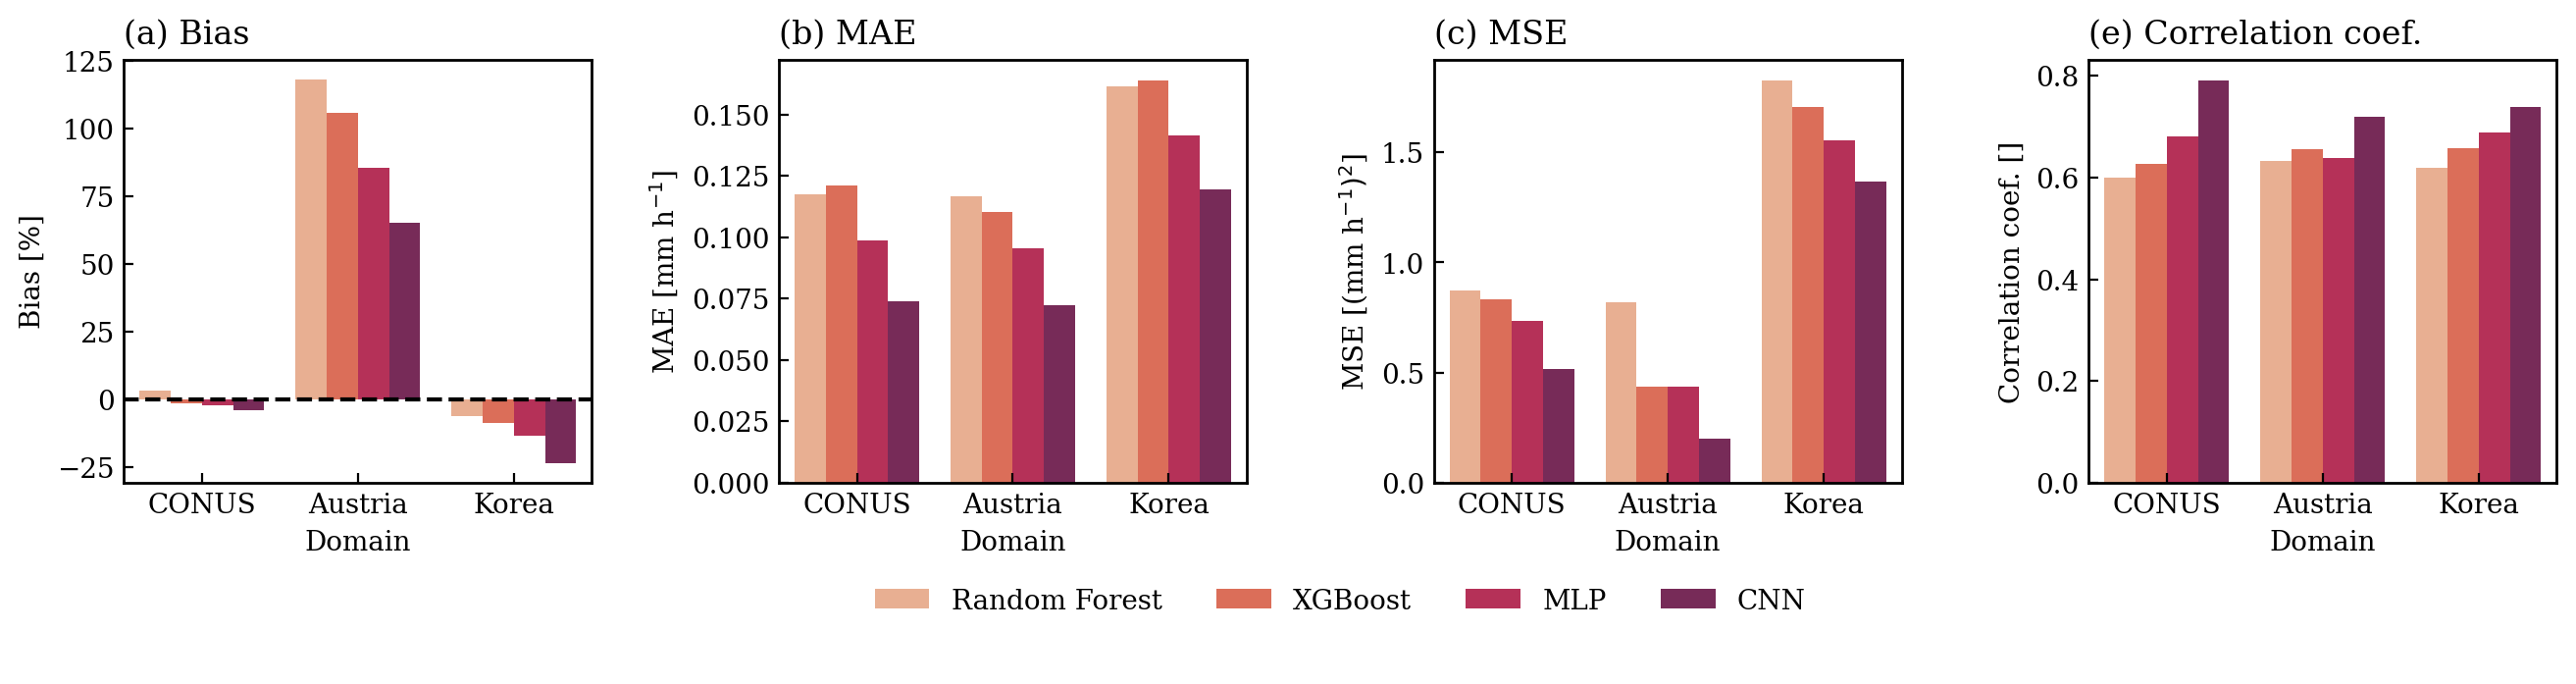
\includegraphics[width=1.0\textwidth]{figures/fig11}
	\caption{
	  Like Fig. 8 but for four different machine-learning techniques trained on GMI observations.
	}
	\label{fig:sensor_comparison}
\end{figure}

Taken together, these results highlight the value of SatRain as a benchmark
dataset: it not only supports the development of precipitation retrievals but
also enables systematic evaluation and comparison of different ML
techniques. We anticipate it will serve as a key resource for researchers aiming
to develop novel retrieval methods.

\section{Usage Notes}

Different scientific and societal applications may require precipitation
retrievals to emphasize specific characteristics, such as convective or frozen
precipitation. While no single benchmark can serve every possible use case, the
SatRain dataset defines five distinct evaluation tasks designed to test the
ability of ML algorithms to reproduce key aspects of precipitation
events. These tasks include: (1) precipitation rate estimation, (2)
probabilistic detection of precipitation, (3) deterministic detection of
precipitation, (4) probabilistic detection of heavy precipitation, and (5)
deterministic detection of heavy precipitation. We adopt thresholds of 0.1 mm/h
and 10 mm/h to define precipitation and heavy precipitation, respectively.
Figure 10 illustrates example results for each of these tasks using the GMI
retrieval presented in the previous section.


\begin{figure}[htbp]
	\centering
	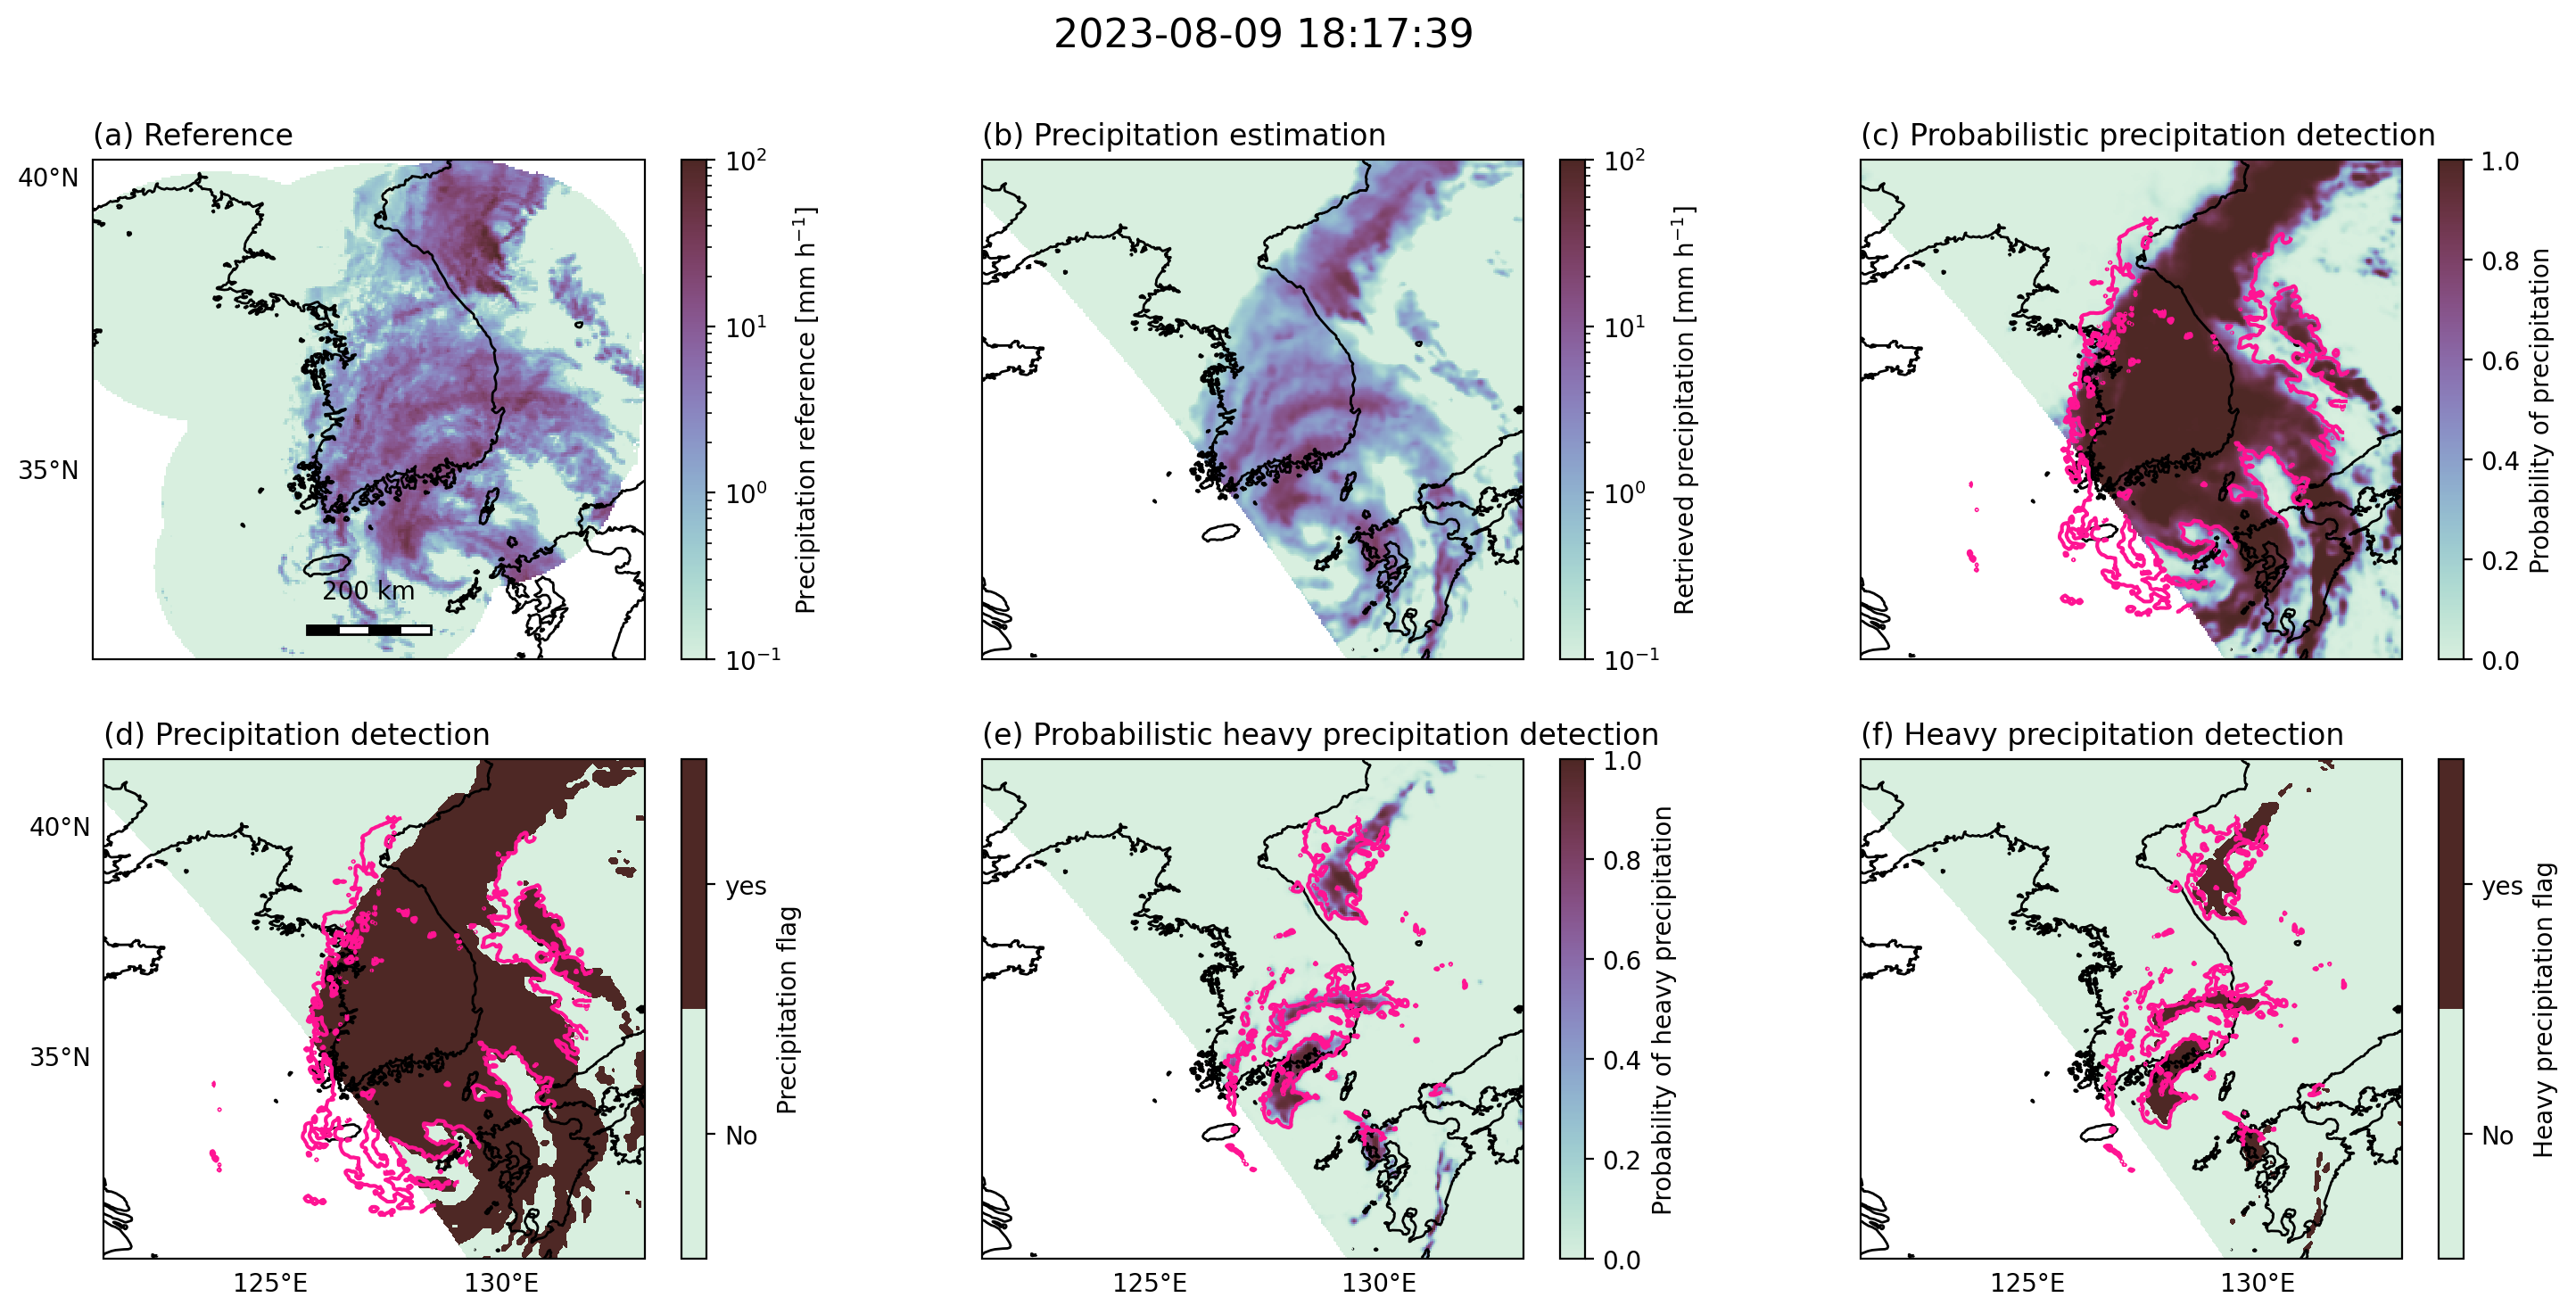
\includegraphics[width=1.0\textwidth]{figures/fig12}
	\caption{
 Example retrieval results for the five suggested precipitation estimation and
 detection tasks during landfall of Typhoon Khanun on August 9, 2023. Panel (b)
 shows quantitative precipitation estimates retrieved from GMI passive microwave
 imager. Panel (c) shows the probability of precipitation for the probabilistic
 precipitation detection task. Panel (d) shows the precipitation flag for the
 deterministic precipitation detection task. Panel (e) and (f) show the
 corresponding probabilistic and deterministic results for the detection of
 heavy precipitation, defined as precipitation exceeding $\SI{10}{\milli \meter \per \hour}$.
	}
	\label{fig:sensor_comparison}
\end{figure}


\subsection{Evaluation Protocol}

To ensure fair comparison of precipitation retrievals trained on the SatRain
dataset, it is essential that models are evaluated using a consistent set of
criteria. We therefore propose a standardized evaluation protocol for
benchmarking ML retrievals on the SatRain dataset. Users may
choose to evaluate their models on all or a subset of the defined tasks. For
each task, the recommended accuracy metrics are listed in Table 4:

A reference implementation of this protocol is available in the ipwgml package.
By default, the evaluation compares all retrieval outputs against the reference
precipitation estimates on the 0.036° regular latitude-longitude grid, ensuring
results are independent of the retrieval’s native coordinate system. For the
CONUS domain, evaluations should be restricted to regions with a radar-quality
index of at least 0.5 and should include both snow and hail.


\subsection{The \texttt{ipwgml} package}

To simplify access to SatRain and accelerate adoption by the community, we have
developed the ipwgml Python package. The package provides utilities to automate
dataset download and management, ensuring that users can begin working with the
dataset without the overhead of manual data handling. Comprehensive
documentation is available at ipwgml.readthedocs.org including installation
instructions, usage examples, and tutorials.

Beyond data access, the package implements the standardized evaluation protocol
defined for SatRain. This functionality allows users to benchmark retrieval
models trained directly on SatRain, as well as to assess independently developed
retrievals against the same criteria. In doing so, the ipwgml package ensures
that evaluation results are reproducible, consistent, and directly comparable
across studies.

\subsection{Limitations}

The SatRain dataset is constructed from high-quality input datasets using
state-of-the-art techniques designed to reduce uncertainties in both the
satellite observations and the precipitation reference. Despite these efforts,
residual uncertainties and measurement errors remain in both components.

On the input side, obviously corrupted satellite imagery is flagged and removed
from the satellite-observation data used to construct the SatRain dataset.
However, more subtle issues such as undetected artifacts or gradual changes in
sensor characteristics may persist and affect the data. These represent
practical challenges that any precipitation retrieval must contend with
warranting their inclusion in the SatRain dataset.

The precipitation reference data are also subject to significant uncertainties.
While gauge-corrected, ground-based radar composites are widely regarded as the
most reliable spatially continuous precipitation estimates currently available,
they are not error-free. Beam overshooting, uncertainties in microphysical
processes, and the particular difficulty of estimating snowfall introduce
systematic biases. Snowfall poses a notable challenge: most gauges do not
accurately measure snow, and MRMS does not apply gauge correction to snowfall
estimates. Consequently, snowfall included in SatRain training and testing data
should be regarded as highly uncertain. For the WegenerNet test data, only
heated gauges are used under likely snowfall conditions, but limitations remain.

To reduce the impact of these uncertainties on retrieval evaluation, SatRain
includes independent test datasets from geographically distinct domains that
rely on entirely independent measurement systems. Performance gains that
transfer to these independent datasets are more likely to reflect genuine
improvements in retrieval capability, rather than overfitting to the same
reference data used in training.

It is also important to note that the primary purpose of SatRain is to serve as
a benchmark for evaluating and comparing retrieval algorithms, rather than as a
basis for developing globally accurate precipitation retrievals. The SatRain
dataset is limited to training data over the CONUS and is therefore not designed
for the development of global precipitation retrievals. Algorithms trained on
SatRain will learn to capture regional precipitation characteristics specific to
North America, which may result in substantial biases or retrieval errors when
applied to other parts of the world.

\subsection{Future Directions}

The SatRain dataset represents the first AI-ready benchmark for satellite-based
precipitation estimation and detection, marking an important step toward
facilitating the operational adoption of ML-based retrievals. It
brings together a comprehensive set of satellite observation types alongside
high-quality precipitation reference data derived according to best practices
agreed upon by the international community. By providing a common reference
point, SatRain enables systematic assessment of ML advances in
precipitation retrieval, improving the comparability, reproducibility, and
eventual uptake of retrieval techniques reported in the scientific literature.

Looking ahead, SatRain also opens opportunities for advancing retrieval science
beyond single-sensor approaches. Its multi-sensor, multi-timestep design
provides a strong foundation for developing next-generation algorithms that fuse
observations across sensors and time steps to better capture precipitation
structure and evolution. Furthermore, the dataset is ideally suited for tackling
broader challenges in global precipitation retrieval, including the development
of sensor-agnostic retrievals and the mitigation of regional biases. By
providing a common starting point to address these challenges, SatRain can help
guide the community toward more robust, transferable, and operationally relevant
precipitation retrieval systems.


\bibliographystyle{plainnat}
\bibliography{bibliography}
\end{document}
